% interactnlmsample.tex
% v1.05 - August 2017

% \documentclass[]{interact}
\documentclass[uplatex,dvipdfmx,a4paper]{book}
\usepackage[top=30mm, bottom=35mm, left=30mm, right=30mm]{geometry}
\usepackage{amsthm}
\usepackage{amssymb}
\usepackage{comment}

\usepackage{epstopdf}% To incorporate .eps illustrations using PDFLaTeX, etc.
\usepackage[caption=false]{subfig}% Support for small, `sub' figures and tables
%\usepackage[nolists,tablesfirst]{endfloat}% To `separate' figures and tables from text if required
%\usepackage[doublespacing]{setspace}% To produce a `double spaced' document if required
%\setlength\parindent{24pt}% To increase paragraph indentation when line spacing is doubled

\usepackage{graphicx}
\usepackage{cite}
\usepackage{algorithm}
\usepackage{algorithmic}
\usepackage{color}
\usepackage{amsmath}
\usepackage{url}

\usepackage[numbers,sort&compress]{natbib}% Citation support using natbib.sty
\bibpunct[, ]{[}{]}{,}{n}{,}{,}% Citation support using natbib.sty
\renewcommand\bibfont{\fontsize{10}{12}\selectfont}% Bibliography support using natbib.sty
\makeatletter% @ becomes a letter
\def\NAT@def@citea{\def\@citea{\NAT@separator}}% Suppress spaces between citations using natbib.sty
\makeatother% @ becomes a symbol again

\theoremstyle{plain}% Theorem-like structures provided by amsthm.sty
\newtheorem{theorem}{Theorem}[section]
\newtheorem{lemma}[theorem]{Lemma}
\newtheorem{corollary}[theorem]{Corollary}
\newtheorem{proposition}[theorem]{Proposition}

\theoremstyle{definition}
\newtheorem{definition}[theorem]{Definition}
\newtheorem{example}[theorem]{Example}

\theoremstyle{remark}
\newtheorem{remark}{Remark}
\newtheorem{notation}{Notation}

\newcommand{\argmax}{\mathop{\rm argmax}\limits}
\newcommand{\argmin}{\mathop{\rm argmin}\limits}

\renewcommand{\baselinestretch}{1.1}
\normalsize

\begin{document}

% \articletype{ARTICLE}% Specify the article type or omit as appropriate

\title{Technical Notes on LiDAR--Inertial SLAM}
\author{Naoki Akai%
  \thanks{Nagoya University, LOCT Co., Ltd.}
}

\maketitle

% \begin{abstract}
% 
% \end{abstract}

% \begin{keywords}
% LiDAR-Inertial Odometry, SLAM,
% \end{keywords}


\section*{Preface}

I have been engaged in research on autonomous navigation of mobile robots since joining my laboratory in 2011.
At that time, 3D LiDAR was not yet common; when people said ``LiDAR,'' they generally meant 2D LiDAR.
For localization using 2D LiDAR, Monte Carlo Localization (MCL) \cite{DellaertICRA1999} was the mainstream method.
MCL is a particle filter-based approach and belongs to the family of probabilistic methods.
Because it is relatively easy to implement and highly extensible, I have mainly focused my research on probabilistic localization methods using MCL.
In particular, I have worked on proposing new frameworks centered around 2D LiDAR.
If I may be a little self-promotional, one of my representative works is the following paper \cite{AkaiJFR2023}.

However, in the broader robotics community, 3D LiDAR was becoming the standard.
Around 2023, I was approached by a company asking whether it would be possible to develop an LIO system using 3D LiDAR.
Although I was familiar with the term LIO, I had not been closely following its research.
To start, I read the well-known FAST LIO paper \cite{FAST-LIO}.
My first impression after reading it was simply, ``I don't understand.''
The paper assumed knowledge of Lie groups and Lie algebras as if it were common sense, and for someone without that background, it was incomprehensible.
However, I also realized that what FAST LIO achieved was remarkable, so I decided to work through it.
After about six months of study, I managed to understand the minimum essentials and became able to implement LIO.

Still, implementing LIO alone did not result in clean maps.
From there, I also implemented graph-based SLAM using Lie groups.
After more than a year, I felt I had finally acquired at least the foundational understanding of LIO and SLAM with Lie groups.
Based on this experience, I decided to reorganize and reimplement the functionality of LIO and SLAM, which led to the development of {\it plain\_slam\_ros2}\footnote{\url{https://github.com/NaokiAkai/plain_slam_ros2}}.
SLAM software--especially LIO and related systems--tends to become very large and complex, making it difficult for newcomers to explore the code.
In contrast, {\it plain\_slam\_ros2} was designed to be relatively compact and well-organized.
After creating {\it plain\_slam\_ros2}, I decided to compile all the knowledge I had used into a single reference, in the hope that it would serve as a resource for those studying LiDAR SLAM in the future.
That was the motivation behind writing this book\footnote{I refer to it as a ``book,'' but please note that it has not undergone formal external review, so there may be errors.}.

To understand this book, the following mathematical knowledge is assumed as prerequisites:
%
\begin{itemize}
  \item Linear algebra (matrix operations, rotation matrices, rigid transformations)
  \item Calculus (partial derivatives of multivariable functions, Jacobians)
\end{itemize}
%
Additionally, the following knowledge will deepen your understanding:
%
\begin{itemize}
  \item Probability and statistics (Gaussian distribution, maximum likelihood estimation)
  \item Numerical optimization (nonlinear least squares)
  \item Lie groups and Lie algebras (${\rm SO}(3)$, ${\rm SE}(3)$ and their exponential/logarithmic maps)
\end{itemize}
%
That said, the minimum necessary mathematical background required to follow this book is summarized in Chapter~\ref{chap:数学的知識}.


\chapter{はじめに}

\section{背景知識}

ロボットの自律移動や自動車の自動運転を行うにあたっては,地図を構築し,その地図上で走行している位置を認識する技術,いわゆる{\bf 自己位置推定}(Localization)や{\bf Simultaneous Localization and Mapping}(SLAM)とよばれる技術が重要であるとされています\cite{Thrun:2005:PR:1121596}.
従来,これらの技術を用いる場合は,{\bf オドメトリ}(Odometry)と呼ばれる移動量推定を行う枠組みが用いられていました.
自己位置推定やSLAMで用いられている技術を端的に述べると,構築された地図(SLAMの場合はオンラインで構築している地図)と,センサの観測値を照合することで,地図上のどの位置に自分が存在しているかを認識する技術になります.
この「センサの観測値と地図の照合」を行うにあたり,オドメトリから予測された移動量を用いることで,どの程度移動したかを予測することが可能となり,照合を行う際の探索範囲を限定することができるようになります.
そのためオドメトリを用いると,自己位置推定およびSLAMの精度や頑健性を向上させることができます.

しかしオドメトリを用いるとなると,自己位置推定やSLAMで用いられる外界センサ(LiDARやカメラ)以外のセンサが必要になります\cite{BorensteinJRS1997}.
オドメトリシステムを構築する上で最も簡単な方法(システムを構築する手間が最もかからないという意味で)は,{\bf Inertial Measurement Unit}(IMU)を用いることだといえます.
IMUは,センサを原点とした加速度と角速度を計測できるセンサであり,これらの値を積分していくだけで移動量を計算することができます.
しかしIMUの計測値が含む誤差は大きく,単に積分して得られた位置や角度の精度は極めて低く,自己位置推定やSLAMには利用できないことがほとんどです.
そのため,IMUだけを用いてオドメトリシステムを構築することは不可能に近いといえます.

移動ロボットや自動運転の分野で最も広く使われているオドメトリシステムは,エンコーダ等を用いて車輪の回転量を計測し,その結果を積分することで移動量を計算する方法です.
これは{\bf ホイールオドメトリ}(Wheel Odometry)と呼ばれます.
ホイールオドメトリを用いれば,タイヤの空転等が発生しない限り,短距離であれば移動量を正確に計測することができます.
ただしホイールオドメトリを用るには,外界センサだけでなく,移動体のハードウェアにも大きな変更を加える必要がります.
そのためホイールオドメトリは,安易に利用できるシステムとは言い難いです.
またホイールオドメトリは,車輪の回転量を計測することが前提のため,基本的に車輪型の移動体にしか適用することができません.

ホイールオドメトリに頼らない移動量の推定方法として,{\bf ビジュアルオドメトリ}(Visual Odometry)が提案されました\cite{VisuailOdometry}.
ビジュアルオドメトリとは,画像から得られる特徴を追跡することで移動量を推定する方法です.
そのためビジュアルオドメトリは,車輪型以外の移動体にも適用することが可能です.
しかし一般に,ビジュアルオドメトリの精度はホイールオドメトリ程高くはないことが知られています.

同様にLiDARを用いて移動量推定を行う方法も様々研究されていましたが,本格的に{\bf LiDAR Odometry}(LO)という言葉が使われた始めた代表的な手法としてLiDAR Odometry and Mapping(LOAM)があります\cite{LOAM}.
LOでは,LiDARが計測する点群を逐次的に照合していくことで移動量の推定を行います.
LiDARの距離計測の精度は高いため,LOによる移動量推定の精度は高くなります.
そのためLOは,様々な用途で使われるようになりました.

しかしLOにも弱点がありました.
LiDAR,特に3D LiDARの計測周期は遅く(一般に$10 \sim 20~{\rm Hz}$程度),高速な動き,特に回転を含む移動量を推定することは困難でした.
この問題を解決する方法として提案されたのが,LiDARとIMUを融合して移動量推定を行う{\bf LiDAR--Inertial Odometry}(LIO)です.
IMUは高周期(一般に100~Hz以上)で加速度と角速度を計測することができるため,LiDARの計測周期の移動量を補間することができます.
この移動の補間を用いると,高速に移動するLiDARによって歪んでしまったLiDARの計測点群を補正することができるようになります.
またLIOでは,LOでは推定されていなかった状態量(速度やIMUの計測値のバイアス)の推定も行います.
そのため,IMUの計測値の積分も正確に行えるようになるため,移動量の推定をより高精度に行うことが可能になりました.
なおVisionとIMUを融合した{\bf Visual--Inertial Odometry}(VIO)は,LIOよりも少し早く提案されていました(例えば\cite{VIO}).









\section{LIOの性能と限界}

LIOのアルゴリズムの進化は目覚ましいものがありましたが,LiDARの性能自体もここ数年で大きく進化しました.
一昔前(著者が研究を始めたのが2011年)では,「LiDARは価格コストが高いため,カメラを用いた手法を提案する」というのが論文等では常套文句でした.
しかし今では,日本円で10万円程度で購入可能な3D LiDARも発売されています.
そして驚くことに,このような価格の3D LiDARでも,360度100~mに近いレンジを計測できるようになっており,LIOを用いて高精度な移動量推定を行うということはかなり一般的になってきました.
そしてLIOを用いるだけでも,小規模な環境であれば十分な精度の点群地図を構築することができるようになりました.
そのため,ドローンのような飛翔体にこのような小型のLiDARを搭載し,高精度な点群地図を生成することも容易に行われるようになってきました.

ただしLIOはあくまでオドメトリシステムであるため,移動量推定しか行いません.
そのため,どれだけ高精度に移動量が推定できたとしても,推定量に誤差(ドリフト)が含まれてしまうため,LIOだけを用いて大規模な環境の地図構築を行うことは依然として難しいです.
特に大規模でループ(一度通過した地点を再度通過すること)が含まれる環境や条件ですと,整合性の取れた地図が構築できなくなってしまいます(同じものが同じ地点に正しくマッピングされなくなります).
前述したSLAMでは,このようなループが含まれる場合であっても,整合性が取れた地図構築を行うことを目的としています.
すなわち,精度の高い地図を構築したい場合には,SLAMの利用は避けられません.

またLIOはあくまで移動量推定のシステムです.
応用上においては,移動量がわかるだけでは嬉しさがあることは少ないといえ,SLAMで構築した地図上で,どの位置にいるかを知れることの方が恩恵が多いといえます.
例えば工場等でAGVやフォークリフトの位置を管理したい場合などには,LIOの利用だけでは不十分であり,自己位置推定の利用が求められます.
そのため,単に高精度のLIOが利用可能になったというだけでは新たな応用システムを提案することは難しく,LIOに含まれるアルゴリズムを正しく理解し,それをSLAMや自己位置推定にも応用していくことが重要になります.





\section{既存手法と本書の立ち位置}

LIOやSLAMを行うオープンソースはすでに多数存在しています.
例えばLIOの有名なオープンソースとしてはLIO-SAM~\cite{liosam2020shan}やFAST-LIO~\cite{FAST-LIO2}が挙げられます.
これらの手法の性能は極めて高く,これらをダウンロードして使用するだけでも,十分な移動量推定を行うことができるといえます.
またLIO-SAMにはSLAMの機能も含まれているため,地図構築を行うこともできます.
またLiDAR SLAMの有名なオープンソースとしては,GLIM~\cite{KoideRAS2024}が挙げられます.
これらの性能も極めて高く,様々な環境で極めて精度の高い点群地図を構築することができます.

しかし多くのソースコードは,機能を多く含むため,どうしても規模が大きくなってしまいます.
そのため,初めてSLAMを学ぼうとする人がこれらを見ても,どこから何を追えば良いかの判断が難しく,結局ダウンロードして使うだけになってしまうことが多いと思います.
本書,および対応するソースコードは,ソフトウェアの構成をとにかくシンプルに実装することに重きをおいています.
開発したソースコードは,LIO,SLAM,自己位置推定の機能を有しており,その主な処理は空行を除いて2000行未満のC++で完結しています.
このC++の中に,スキャンマッチング,LiDARとIMUの融合(ルーズカップリングとタイトカップリング),ループ検知,ポーズグラフの最適化といった必要な処理をすべて実装しています(用語の詳細は後ほど解説します).
また依存ライブラリも極力少なくし,ほぼフルスクラッチでLIOやSLAMを実装できるようになるようにしています.
なお,主な依存ライブラリは{\it Sophus}({\it Eigen}ベース)と{\it nanoflann}のみになります(他はパラメーター設定のために{\it YAML}を用いています).
これらはそれぞれ線形・リー代数を扱うライブラリと,最近某探索を行うライブラリとなっており,LIOやSLAMの根幹となる部分はすべてフルスクラッチで実装されているため,初学者でもどのように最適化などが実装されているか理解しやすい構成になっていると思います.



\chapter{数学的知識}
\label{chap:数学的知識}

\section{表記}

本書では基本的に実数しか扱いません.
そのため断りのない限り,実数が使われていることを前提とします.
表記としては,スカラーを$a \in \mathbb{R}$,$N$次元のベクトルを${\bf a} \in \mathbb{R}^{N}$,$N \times M$の行列を$A \in \mathbb{R}^{N \times M}$と表記します.
また単位行列をよく用いますが,次元をわかりやすくするために添え字を付けます.
例えば$N$次元の単位行列は$I_{N}$と示します.













\section{ヤコビアン}

本書では主に{\bf 最適化}(Optimization)を利用していきます.
最適化とは,ある変数${\bf x} = \left( x_{1} ~ \cdots ~ x_{N} \right)^{\top} \in \mathbb{R}^{N}$に従う関数$f({\bf x})$(最適化に使われる関数はよく{\bf コスト関数}(Cost Function)と呼ばれます)が定義されたときに,$f$の値を最小化(もしくは最大化)させること,またそれに対応する変数${\bf x}$を求めることになります.
最適化を行う方法には様々な方法がありますが,基本となることは,関数の勾配を求めることになり,これは式(\ref{eq:scholar_function_jacobian})で定義されます.
%
\begin{align}
  \frac{ \partial f({\bf x}) }{ \partial {\bf x} } =
  \left( \begin{matrix}
    \frac{ \partial f({\bf x}) }{ \partial x_{1} } &
    \cdots                                         &
    \frac{ \partial f({\bf x}) }{ \partial x_{N} }
  \end{matrix} \right)
  \label{eq:scholar_function_jacobian}
\end{align}
%
なお,関数を引数であるベクトルで偏微分した結果は,{\bf ヤコビアン}(Jacobian)と呼ばれます.
ベクトル関数${\bf f}({\bf x}) = \left( f_{1} \left( {\bf x} \right) ~ \cdots ~ f_{M} \left( {\bf x} \right) \right)^{\top} \in \mathbb{R}^{M}$に関してもヤコビアンを定めることができ,これは式(\ref{eq:vector_function_jacobian})で表すことができます.
%
\begin{align}
  \frac{ \partial {\bf f} \left( {\bf x} \right) }{ \partial {\bf x} } =
  \left( \begin{matrix}
    \frac{ \partial f_{1} \left( {\bf x} \right) }{ \partial x_{1} } &
    \cdots                                             &
    \frac{ \partial f_{1} \left( {\bf x} \right) }{ \partial x_{N} } \\
    %
    \vdots                                             &
    \ddots                                             &
    \vdots                                             \\
    %
    \frac{ \partial f_{M} \left( {\bf x} \right) }{ \partial x_{1} } &
    \cdots                                             &
    \frac{ \partial f_{M} \left( {\bf x} \right) }{ \partial x_{N} } \\
  \end{matrix} \right)
  \label{eq:vector_function_jacobian}
\end{align}
%
なお本書では,基本的にヤコビアンを$J$と表記します.

ヤコビアンの計算は基本的に式(\ref{eq:scholar_function_jacobian}),(\ref{eq:vector_function_jacobian})に示す定義に従って行いますが,少し異なった方法でも導出することが可能であり,本書では基本的にこの方法を用いてヤコビアンを求めていきます.
まず,関数$f \left( {\bf x} \right)$を$\delta {\bf x}$だけ変化させた結果をテイラー展開を用いて近似します.
%
\begin{align}
  f \left( {\bf x} + \delta {\bf x} \right) \simeq
  f \left( {\bf x} \right) + 
  J \delta {\bf x} + 
  \frac{1}{2} \delta {\bf x}^{\top} H \delta {\bf x}
  \label{eq:taylor_expansion_approximation_2nd_order}
\end{align}
%
なお$H = \partial^{2} f \left( {\bf x} \right) / \partial {\bf x}^{2}$であり,これは{\bf ヘッセ行列}(Hessian)と呼ばれます.
ここで,2次の微小量を無視し,式(\ref{eq:taylor_expansion_approximation_2nd_order})の両辺が等しいと仮定すると,次式が得られます.
%
\begin{align}
  f \left( {\bf x} + \delta {\bf x} \right) - f \left( {\bf x} \right) = J \delta {\bf x}
  \label{eq:jacobian_difference}
\end{align}
%
すなわち,$f \left( {\bf x} + \delta {\bf x} \right)$と$f \left( {\bf x} \right)$の差分を$J \delta {\bf x}$という形で記述できるとヤコビアンを求めることができます.

例えば,$f \left( x \right) = x^{2}$という簡単な例を考えてみます.
この関数のヤコビアン\footnote{正確には引数がスカラーなので導関数と呼ぶのが一般的ですが,1次元の場合のヤコビアンと形式的に見なすことができます.}は$\partial x^{2} / \partial x = 2x$となりますが,式(\ref{eq:jacobian_difference})に示す方法でヤコビアンを求めてみます.
%
\begin{align}
  \begin{split}
    (x + \delta x)^{2} - x^{2}
    = & x^{2} + 2 x \delta x + \delta x^{2} - x^{2} \\
    = & 2 x \delta x
  \end{split}
  \label{eq:jacobian_difference_example}
\end{align}
%
ただし,$\delta x^{2} \simeq 0$として2次の微小量を無視しました.  
式(\ref{eq:jacobian_difference_example})に示すように,$f \left( x \right) = x^{2}$のヤコビアンを正しく求めることができました.
この方法を用いると,関数を直接微分しなくても,ヤコビアンを求めることができます\footnote{ここで得られるヤコビアンは,関数をテイラー展開し,2次以上の微小項を無視することで得られる1次近似により得られたものです.$\delta x \to 0$ の極限では,理論的な微分(導関数)と一致しますが,有限の差分を用いる場合は数値的な近似値となります.}.













\section{ガウス・ニュートン法}
\label{subsec:gauss-newton_method}

本書で扱う問題は,度々最適化問題に帰着されます.
最適化問題を解く際に用いられる方法は様々ありますが,本書では{\bf ガウス・ニュートン法}(Gauss-Newton Method)を主に用います.

ガウス・ニュートン法を考えるにあたり,まず状態変数${\bf x} \in \mathbb{R}^{N}$,およびこの状態に依存する{\bf 残差}(Residual)(もしくは残差ベクトル)${\bf r} \left( {\bf x} \right) \in \mathbb{R}^{M}$を導入します.
今,複数の残差ベクトルを用いて,以下のコスト関数を定義します.
%
\begin{align}
  E \left( {\bf x} \right) = \sum_{i} \| {\bf r}_{i} \left( {\bf x} \right) \|_{2}^{2} \in \mathbb{R}
\end{align}
%
ここで$\| \cdot \|_{2}^{2}$は,ベクトルのユーグリッドノルムの2乗を計算する操作です.
そして,コスト関数を最小化する状態を以下のように定義します.
%
\begin{align}
  {\bf x}^{*} = \argmin_{ {\bf x} } E \left( {\bf x} \right)
\end{align}
%
これは,${\bf x}$の定義域においてコスト関数 $E \left( {\bf x} \right)$を最小にするような状態${\bf x}^{*}$を求めることを意味します.
このような解は,{\bf 最適解}(Optimal Solution)と呼ばれます.

ガウス・ニュートン法による最適化を考えるにあたり,まず残差ベクトルを1次のテイラー展開で近似することを考えます.
%
\begin{align}
  {\bf r} \left( {\bf x} + \delta {\bf x} \right) \simeq {\bf r} \left( {\bf x} \right) + J \delta {\bf x}
  \label{eq:error_vector_taylor}
\end{align}
%
ここで$J$は残差ベクトル${\bf r}$の状態ベクトル${\bf x}$に関するヤコビアン$\partial {\bf r} / \partial {\bf x} \in \mathbb{R}^{M \times N}$になります.
次に,式(\ref{eq:error_vector_taylor})の近似された残差ベクトルの2乗ノルムを考えます.
%
\begin{align}
  \begin{split}
    \left( {\bf r} + J \delta {\bf x} \right)^{\top} \left( {\bf r} + J \delta {\bf x} \right)
    %
    = & \left( {\bf r}^{\top} + \delta {\bf x}^{\top} J^{\top} \right) \left( {\bf r} + J \delta {\bf x} \right) \\
    %
    = & {\bf r}^{\top} {\bf r} + {\bf r}^{\top} J \delta {\bf x} + \delta {\bf x}^{\top} J^{\top} {\bf r} + \delta {\bf x}^{\top} J^{\top} J \delta {\bf x} \\
    %
    = & {\bf r}^{\top} {\bf r} + 2 \delta {\bf x}^{\top} J^{\top} {\bf r} + \delta {\bf x}^{\top} J^{\top} J \delta {\bf x}
  \end{split}
  \label{eq:error_vector_taylor_sq_norm}
\end{align}
%
なお,${\bf r}^{\top} J \delta {\bf x} = \delta {\bf x}^{\top} J^{\top} {\bf r}$を用いています.

続いて,式(\ref{eq:error_vector_taylor_sq_norm})を$\delta {\bf x}$の関数$f \left( \delta {\bf x} \right)$とみなして,$\delta {\bf x}$で偏微分します.
%
\begin{align}
  \frac{ \partial f \left( \delta {\bf x} \right) }{ \partial \delta {\bf x} } = 2 J^{\top} {\bf r} + 2 J^{\top} J \delta {\bf x}
  \label{eq:error_vector_taylor_sq_norm_partial}
\end{align}
%
そして,式(\ref{eq:error_vector_taylor_sq_norm_partial})が${\bf 0}$になると仮定すると,次式が成り立ちます.
%
\begin{align}
  J^{\top} J \delta {\bf x} = -J^{\top} {\bf r}
  \label{eq:gauss_newton_update_value}
\end{align}

ここで,式(\ref{eq:gauss_newton_update_value})を満たす$\delta {\bf x}$について考えます.
$f \left( \delta {\bf x} \right)$は,$\delta {\bf x}$だけ状態を変化させたときの残差ベクトルを近似し,その2乗ノルムを計算したものになっています.
これを$\delta {\bf x}$に関して偏微分し,その結果を${\bf 0}$とすると,近似した残差ベクトルの2乗ノルムを最小にする$\delta {\bf x}$を求めることが可能になります.
すなわち,この操作で求められた$\delta {\bf x}$分だけ${\bf x}$を更新すると,コスト関数を減少させることができるようになります.

式(\ref{eq:error_vector_taylor_sq_norm})を導出するにあっては,1つの残差ベクトルの近似を考えましたが,実際のコスト関数では複数の残差ベクトルの2乗ノルムの和を計算しています.
そのため,状態${\bf x}$を$\delta {\bf x}$だけ変化させたコスト関数を近似する必要がありますが,これは式(\ref{eq:cost_function_taylor})のようになります.
%
\begin{align}
  E \left( {\bf x} + \delta {\bf x} \right) \simeq \sum_{i} \left( {\bf r}_{i}^{\top} {\bf r}_{i} + 2 \delta {\bf x}^{\top} J_{i}^{\top} {\bf r}_{i} + \delta {\bf x}^{\top} J_{i}^{\top} J_{i} \delta {\bf x} \right)
  \label{eq:cost_function_taylor}
\end{align}
%
そして同様に,式(\ref{eq:cost_function_taylor})を$\delta {\bf x}$で偏微分した結果を${\bf 0}$にすると,次式が得られます.
%
\begin{align}
  \sum_{i} J_{i}^{\top} J_{i} \delta {\bf x} = -\sum_{i} J_{i}^{\top} {\bf r}_{i}
  \label{eq:gauss_newton_update_sum}
\end{align}
%
ここで簡略化のため,以下のように変数を導入します.
%
\begin{align}
  \begin{gathered}
    H = \sum_{i} J_{i}^{\top} J_{i} \\
    {\bf b} = \sum_{i} J_{i}^{\top} {\bf r}_{i}
  \end{gathered}
  \label{eq:hessian_and_gradient_gauss_newton}
\end{align}
%
これにより式(\ref{eq:gauss_newton_update_sum})は$H \delta {\bf x} = -{\bf b}$と書けます.
なおこの$H$と${\bf b}$はそれぞれヘッセ行列と勾配とも呼ばれます.
ガウス・ニュートン法を用いた最適化では,$H \delta {\bf x} = -{\bf b}$を満たす$\delta {\bf x}$を得た後に,以下のように状態を更新します.
%
\begin{align}
  {\bf x} \leftarrow {\bf x} + \delta {\bf x}
  \label{eq:gauss_newton_update_vector}
\end{align}
%
なお,$H \delta {\bf x} = -{\bf b}$からは,当然$\delta {\bf x} = -H^{-1} {\bf b}$が導けますが,$H \in \mathbb{R}^{N \times N}$になるため,$N$が大きい場合には逆行列の直接的な計算が困難になります.
そのため,直接逆行列を計算することが少ないため,「$H \delta {\bf x} = -{\bf b}$を満たす$\delta {\bf x}$」という表現を用いています.
$N$が大きくない場合は,直接$H^{-1}$を計算しても実用上は問題になりません.









\section{ロバストカーネル}

最適化を実行するにあたり,残差ベクトルを複数定義しますが,誤った対応,すなわち誤対応を用いて残差ベクトルを定義してしまうと,最適化に悪影響を及ぼすことになります.
通常,誤対応によって生じる残差ベクトルのノルムは,正しい対応に比べて大きくなる傾向があります.
そのため,残差ベクトルのノルムの大きさに応じて最適化への影響を抑制することが有効です.
このような効果を実現するために,{\bf ロバストカーネル}(Robust Kernel)を導入することができます.

一般にロバストカーネルを導入したコスト関数は以下のように記述されます.
%
\begin{align}
  E \left( {\bf x} \right) = \sum_{i} \rho \left( \| {\bf r}_{i} \left( {\bf x} \right) \|_{2}^{2} \right)
  \label{eq:cost_function_robust_kernel}
\end{align}
%
式(\ref{eq:cost_function_robust_kernel})に示す$\rho \left( \cdot \right)$がロバストカーネルになります.
ロバストカーネルにも様々なものがありますが,本書では{\bf フーバー損失}(Huber Loss)を用います.
フーバー損失は以下のように定義されます.
%
\begin{align}
  \rho \left( s \right)
  =
  \begin{cases}
    s                                & {\rm if} ~ s \leq \delta^{2} \\
    2 \delta \sqrt{ s } - \delta^{2} & {\rm otherwise}
  \end{cases}
  \label{eq:huber_loss}
\end{align}
%
ここで$\delta$は任意の正の実数です.

フーバー損失を用いたガウス・ニュートン法を考えるにあたり,式(\ref{eq:error_vector_taylor_sq_norm})に示したように,残差ベクトルの微小変化${\bf r} \left( {\bf x} + \delta {\bf x} \right)$を線形近似した結果,すなわち${\bf r} \left( {\bf x} \right) + J \delta {\bf x}$に対するフーバー損失を考ます.
%
\begin{align}
  \rho \left( \left( {\bf r} + J \delta {\bf x} \right)^{\top} \left( {\bf r} + J \delta {\bf x} \right) \right)
  =
  \rho \left( {\bf r}^{\top} {\bf r} + 2 \delta {\bf x}^{\top} J^{\top} {\bf r} + \delta {\bf x}^{\top} J^{\top} J \delta {\bf x} \right)
\end{align}
%
ここで$s = {\bf r}^{\top} {\bf r} + 2 \delta {\bf x}^{\top} J^{\top} {\bf r} + \delta {\bf x}^{\top} J^{\top} J \delta {\bf x}$とします.
式(\ref{eq:huber_loss})より,$s \leq \delta^{2}$の場合は$s$がそのまま用いられるため,$s$が$\delta^{2}$より大きくなる例を考えることとし,与えられた$s$をフーバー損失に代入した結果を$\delta {\bf x}$で微分します.
%
\begin{align}
  \begin{split}
    \frac{ \partial \rho \left( s \right) }{ \partial \delta {\bf x} }
    = &
    \frac{ \partial \rho \left( s \right) }{ \partial s }
    \frac{ \partial s }{ \partial \delta {\bf x} } \\
    = &
    \frac{ \delta }{ \sqrt{s} } \left( 2 J^{T} {\bf r} + 2 J^{\top} J \delta {\bf x} \right)
  \end{split}
  \label{eq:huber_loss_diff}
\end{align}
%
そして式(\ref{eq:huber_loss_diff})が${\bf 0}$になるとすると,以下が得られます.
%
\begin{align}
  \frac{ \delta }{ \sqrt{s} } J^{\top} J \delta {\bf x} = -\frac{ \delta }{ \sqrt{s} } J^{T} {\bf r}
  \label{eq:gauss_newton_update_value_huber_loss}
\end{align}
%
式(\ref{eq:gauss_newton_update_value})と比較すると,式(\ref{eq:gauss_newton_update_value_huber_loss})では両辺に$\delta / \sqrt{s}$が表れます.
なお式(\ref{eq:gauss_newton_update_value_huber_loss})における$\delta / \sqrt{s}$は削除することができますが,実際には複数の残差ベクトルの和を考えることとなり,この値は考える残差ベクトル毎に異なる値となるため,削除せずに記述しています.

そして,式(\ref{eq:hessian_and_gradient_gauss_newton})に示したように,すべての残差ベクトルを考慮してヘッセ行列と勾配を定めると以下のようになります.
%
\begin{align}
  \begin{gathered}
    H = \sum_{i} \rho^{\prime} \left( s_{i} \right) J_{i}^{\top} J_{i} \\
    {\bf b} = \sum_{i} \rho^{\prime} \left( s_{i} \right) J_{i}^{\top} {\bf r}_{i}
  \end{gathered}
  \label{eq:hessian_and_gradient_gauss_newton_huber_loss}
\end{align}
%
なお$\rho^{\prime} \left( s \right) = \partial \rho \left( s \right) / \partial s$であり,これは式(\ref{eq:huber_loss})より以下となります.
%
\begin{align}
  \rho^{\prime} \left( s \right)
  =
  \begin{cases}
    1                             & {\rm if} ~ s \leq \delta^{2} \\
    \frac{ \delta }{ \sqrt{ s } } & {\rm otherwise}
  \end{cases}
  \label{eq:huber_loss_prime}
\end{align}
%

ただし$s = {\bf r}^{\top} {\bf r} + 2 \delta {\bf x}^{\top} J^{\top} {\bf r} + \delta {\bf x}^{\top} J^{\top} J \delta {\bf x}$としたため,このままで$\rho^{\prime} \left( \cdot \right)$が$\delta {\bf x}$に依存してしまい,ガウス・ニュートン法の線形構造が崩れて式(\ref{eq:gauss_newton_update_sum})に示すような形で状態の更新量を求められなくなってしまいます.
そこで$s_{0} = {\bf r}^{\top} {\bf r}$,$\delta s = 2 \delta {\bf x}^{\top} J^{\top} {\bf r} + \delta {\bf x}^{\top} J^{\top} J \delta {\bf x}$とし,$\rho^{\prime} \left( s \right) \simeq \rho^{\prime} \left( s_{0} \right) + \rho^{\prime \prime} \left( s_{0} \right) \delta s$として近似します.
そして,$\rho^{\prime \prime} \left( s_{0} \right) \delta s$が高次の微小量であるとみなして無視してしまい$\rho^{\prime}(s) \simeq \rho^{\prime}(s_0)$と近似してしまいます.
これにより,$\rho^{\prime} \left( s \right) \simeq \rho^{\prime} \left( s_{0} \right)$とすることができ,$\delta {\bf x}$に依存しない形となるため,ガウス・ニュートン法における線形構造を維持することができます.

最終的に,$w = \rho^{\prime} \left( {\bf r}^{\top} {\bf r} \right)$とする重みを定義し,ヘッセ行列と勾配を以下のように定めます.
%
\begin{align}
  \begin{gathered}
    H = \sum_{i} w_{i} J_{i}^{\top} J_{i} \\
    {\bf b} = \sum_{i} w_{i} J_{i}^{\top} {\bf r}_{i}
  \end{gathered}
  \label{eq:hessian_and_gradient_gauss_newton_huber_loss_weight}
\end{align}
%
これらの$H$と${\bf b}$を用いて$H \delta {\bf x} = -{\bf b}$を満たす$\delta {\bf x}$を求め,式(\ref{eq:gauss_newton_update_vector})に基づき状態更新を行うことで,フーバー損失を用いたガウス・ニュートン法による最適化を実行することができます.
フーバー損失を用いた場合のガウス・ニュートン法による状態更新の導出は少し複雑にはなりますが,実装にあたっては,単に式(\ref{eq:huber_loss_prime})に示す関数を重みとして計算してそれぞれのヘッセ行列と勾配に掛けるだけなので,非常に容易に実装することができます.
また多くの場合,フーバー損失を用いることで最適化がよりロバストになります.
















\section{リー群とリー代数}

本書では頻繁に{\bf リー群}(Lie Group)と{\bf リー代数}(Lie Algebra)を用います.
リー群やリー代数の厳密な説明は行いませんが,本書でリー群と呼んだ場合は{\bf 回転行列}(Rotation Matrix)と{\bf 剛体変換行列}(Rigid Transformation Matrix)を示すこととします.

回転行列は以下のように定義されます.
%
\begin{align}
  \{R \in \mathbb{R}^{3 \times 3} | R^{\top} R = I, {\rm det}(R) = 1\}
  \label{eq:def_SO3}
\end{align}
%
回転行列はSpecial Orthogonal Group in 3 Dimensions(${\rm SO}(3)$)とも呼ばれ,3次元空間の回転を表現することができます.
剛体変換行列は以下のように定義されます.
%
\begin{align}
  \left\{ \left( \begin{matrix} R & {\bf t} \\ {\bf 0}^{\top} & 1 \end{matrix} \right) \in \mathbb{R}^{4 \times 4} | R \in {\rm SO}(3), {\bf t} \in \mathbb{R}^{3} \right\}
  \label{eq:def_SE3}
\end{align}
%
剛体変換行列はSpecial Euclidean Group in 3 Dimensions(${\rm SE}(3)$)とも呼ばれ,3次元空間での回転を含む位置(姿勢)を表現することができます.
LIOやSLAMでは基本的に,${\rm SO}(3)$や${\rm SE}(3)$を用いて状態を表現します.
なお式(\ref{eq:def_SE3})から明らかなように,$T$を構成する変数は${\bf t}$と$R$になります.
そのため,本書ではしばしば$T = \left( R \mid {\bf t} \right)$という簡略表記を用います.

リー群を用いる利点は,回転の状態を,途中で急に値が飛んだり切り替わったりすることなく,滑らかにかつ数学的に自然な形で扱えるということです.
詳細は省きますが,このような空間を{\bf 多様体}(Manifold)と呼びます.
直感的には少し難しく感じるかもしれませんが,まずは平面上の回転,つまり$xy$平面での角度$\theta$を例に考えてみます.
角度$\theta$は通常,$0 \leq \theta < 2\pi$(あるいは$-\pi \leq \theta < \pi$)の範囲で定義されますが,$\theta = 0$と$\theta = 2\pi$は,数値としては異なるものの,回転としては同じ状態を表しています.
このような性質から,角度$\theta$による表現では,状態が不連続に見えることがあります.
しかしリー群を使えば,回転の変化を「切れ目のない空間」で表現でき,最初から最後まで滑らかに(連続的に)扱えるようになります.
また,加減算や微分といった操作も数学的に統一されたルールで行えるので,処理が一貫してスムーズになります.
しかしリー群を用いて状態を表すと,処理が少し直感的なものではなくなってしまいます.

例えばロボットの状態をあるベクトル空間で${\bf x}$と表すとします.
もしロボットの状態が$\Delta {\bf x}$だけ変化したとすると,直感的にはロボットの状態は${\bf x} + \Delta {\bf x}$という,シンプルな加算により求めることができます(ただし前述のような角度$\theta$が含まれる場合は値の範囲に中止いなければなりません).
しかし式(\ref{eq:def_SO3}),(\ref{eq:def_SE3})に示す通り,${\rm SO}(3)$や${\rm SE}(3)$には満たすべき制約があるため,同様の加算を行うとこのような制約を満たさなくなります.

例えば,3次元空間上での並進と回転を含む変化量を$\Delta T \in {\rm SE}(3)$とし,以下のように定めます.
%
\begin{align}
  \Delta T
%
  = \left( \begin{matrix}
      \Delta R       & \Delta {\bf t} \\
      {\bf 0}^{\top} & 1
    \end{matrix} \right)
\end{align}
%
ここで,$T$と$\Delta T$の単純な加算を考えると以下になります.
%
\begin{align}
  T + \Delta T
%
  = \left( \begin{matrix}
      R + \Delta R       & {\bf t} + \Delta {\bf t} \\
      {\bf 0}^{\top}     & 2
    \end{matrix} \right) \notin {\rm SE}(3)
\end{align}
%
これは明らかに式(\ref{eq:def_SE3})を満たさないため,$T + \Delta T$は剛体変換行列にはなりません.
${\rm SE}(3)$の制約を満たしたまま変化を反映させるためには,$T \Delta T$を計算します\footnote{行列の積は左右どちらから掛けるかで結果が変わるため,$\Delta T$をどちらから作用させるかが重要になりますが,本書では基本的に動作に伴う変化に関しては右作用を用います.}.
%
\begin{align}
  T \Delta T
%
  = \left( \begin{matrix}
      R \Delta R     & R \Delta {\bf t} + {\bf t} \\
      {\bf 0}^{\top} & 1
    \end{matrix} \right) \in {\rm SE}(3)
  \label{eq:se3_add}
\end{align}
%
また,$T_{1}, T_{2} \in {\rm SE}(3)$間の差分を$\Delta T$とした場合,$T_{1} \Delta T = T_{2}$となるため,$T_{1}$と$T_{2}$の間の差分は以下のように定義されます.
%
\begin{align}
  \begin{split}
    \Delta T
%
    & = T_{1}^{-1} T_{2} \\
%
    & = \left( \begin{matrix}
          R_{1}^{\top} R_{2} & R_{2} ({\bf t}_{2} - {\bf t}_{1}) \\
          {\bf 0}^{\top}     & 1
        \end{matrix} \right) \in {\rm SE}(3)
  \end{split}
  \label{eq:se3_diff}
\end{align}

式(\ref{eq:se3_add}),(\ref{eq:se3_diff})を用いれば,${\rm SE}(3)$(もしくは${\rm SO}(3)$)の空間での状態の変化を考えることができます.
しかしこれらはベクトル空間で議論される加算や減算と比較すると直感的でなく,また前節までで述べたガウス・ニュートン法が適用できる表現になっていません.
そこで,リー群を用いて表せられている状態をベクトルに対応させなれないかということを考えますが,リー群に対応したベクトル空間としてリー代数を用いることができます.
そして${\rm SO}(3)$,${\rm SE}(3)$に対応したリー代数をそれぞれ$\mathfrak{so}(3)$,$\mathfrak{se}(3)$と記述します.
$\mathfrak{so}(3)$と$\mathfrak{se}(3)$は厳密にはそれぞれ$\mathbb{R}^{3 \times 3}$と$\mathbb{R}^{4 \times 4}$の行列の集合ですが,それぞれ独立した3つと6つの実数で表現することができるため,3次元,および6次元ベクトルとして表現できます.
そして,${\rm SO}(3)$と$\mathfrak{so}(3)$,もしくは${\rm SE}(3)$と$\mathfrak{se}(3)$間を変換させる写像として,それぞれ{\bf 指数写像}(Exponential Map)と{\bf 対数写像}(Logarithm Map)があります.
%
\begin{align}
  \begin{gathered}
    \exp: \mathfrak{so}(3) \rightarrow {\rm SO}(3) \\
    \log: {\rm SO}(3) \rightarrow \mathfrak{so}(3) \\
  \end{gathered}
  \label{eq:so3_exp_log_maps}
\end{align}
%
\begin{align}
  \begin{gathered}
    \exp: \mathfrak{se}(3) \rightarrow {\rm SO}(3) \\
    \log: {\rm SO}(3) \rightarrow \mathfrak{se}(3) \\
  \end{gathered}
  \label{eq:se3_exp_log_maps}
\end{align}
%
なお,式(\ref{eq:so3_exp_log_maps})と式(\ref{eq:se3_exp_log_maps})に示す指数・対数写像はそれぞれ別物になります.
ただし,本書で使用するにあたって適宜${\rm SO}(3)$や${\rm SE}(3)$といった断りは入れないため,引数となっている変数でどちらの写像が使われているか判断します.

リー代数を用いることで,状態量がリー群を用いて表現されている場合でも,ガウス・ニュートン法などを用いた最適化を行うことができますが,リー代数を用いた最適化を述べる前に,指数写像や対数写像について解説します.
ただしこれらの写像の導出はせず,あくまで計算がどのように行われているかだけを示します.











\subsection{指数写像と対数写像}

ある3次元ベクトル$\boldsymbol \phi$に対して,式(\ref{eq:so3_exp_log_maps})に示す指数写像は以下のように定義されます.
%
\begin{align}
  \begin{gathered}
    \theta = \| \boldsymbol \phi \|_{2} \\
    %
    \exp \left( \boldsymbol \phi^{^\wedge} \right)
    =
    I_{3} +
    \frac{ \sin \theta }{ \theta } \boldsymbol \phi{^\wedge} +
    \frac{ 1 - \cos \theta }{ \theta^{2} } \left( \boldsymbol \phi{^\wedge} \right)^{2}
  \end{gathered}
  \label{eq:so3_exp_map}
\end{align}
%
ここで$\left( \cdot \right)^{\wedge}$は,3次元ベクトルを$\mathfrak{so}(3)$に変換する操作(もしくは6次元ベクトルを$\mathfrak{se}(3)$に変換する操作)であり,3次元ベクトルの場合は{\bf 反対称行列}(Skew-Symmetric Matrix)を生成する操作であるともみなせます.
%
\begin{align}
  \boldsymbol \phi^{^\wedge}
%
  = \left( \begin{matrix}
      0         & -\phi_{z} & \phi_{y} \\
      \phi_{z}  & 0         & -\phi_{x} \\
      -\phi_{y} & \phi_{x}  & 0
    \end{matrix} \right) \in \mathfrak{so}(3)
  \label{eq:skew_symmetric_matrix}
\end{align}
%
少し話が逸れますが,反対称行列の持つ性質として,${\bf a}^{^\wedge} {\bf b} = -{\bf b}^{^\wedge} {\bf a}$というものがあります(ただし${\bf a}, {\bf b} \in \mathbb{R}^{3}$です).
%
\begin{align}
  \begin{split}
    {\bf a}^{^\wedge} {\bf b}
%
    & = \left( \begin{matrix}
          -a_{z} b_{y} + a_{y} b_{z} \\
           a_{z} b_{x} - a_{x} b_{z} \\
          -a_{y} b_{x} + a_{x} b_{y}
        \end{matrix} \right) \\
%
    & = \left( \begin{matrix}
          0      &  b_{z} & -b_{y} \\
          -b_{z} & 0      & b_{x} \\
          b_{y}  & -b_{x} & 0
        \end{matrix} \right)
        \left( \begin{matrix}
          a_{x} \\
          a_{y} \\
          a_{z}
        \end{matrix} \right) \\
%
     & = -{\bf b}^{\wedge} {\bf a} 
  \end{split}
\end{align}
%
この性質は,後ほどの実装でヤコビアンを計算するときに用います.

また,式(\ref{eq:so3_exp_log_maps})に示す対数写像は以下のように定義されます.
%
\begin{align}
  \begin{gathered}
    \theta = \arccos \left( \frac{{\rm tr}(R) - 1}{ 2 } \right) \\
    %
    \log( R ) = \frac{ \theta }{ 2 \sin \theta } \left( R - R^{\top} \right)
  \end{gathered}
  \label{eq:so3_log_map}
\end{align}
%
なお$\log \left( R \right) = \boldsymbol \phi^{\wedge} \in \mathfrak{so}(3)$となるため,この反対称行列から3次元ベクトル$\boldsymbol \phi = \left( \phi_{x} ~ \phi_{y} ~ \phi_{z} \right)^{\top}$を取り出す操作を以下のように定義します.
%
\begin{align}
  \boldsymbol \phi = \left( \boldsymbol \phi^{\wedge} \right)^{\vee}
\end{align}
%
後に示しますが,$\mathfrak{se}(3)$から6次元ベクトルを取り出す操作も同様に$\left( \cdot \right)^{\vee}$と表記します.

式(\ref{eq:so3_exp_map}),(\ref{eq:so3_log_map})では,それぞれ$\theta$が分母に表れるため,$\theta \ll 1$の場合計算が不安定になります.
そのため$\theta \ll 1$の場合には,以下のように近似して計算を行います.
%
\begin{align}
  \begin{gathered}
    \exp \left( \boldsymbol \phi^{\wedge} \right) \simeq I_{3} + \boldsymbol \phi^{\wedge} + \frac{1}{2} \left( \boldsymbol \phi^{\wedge} \right)^{2} \\
%
    \log \left( R \right) \simeq \frac{1}{2} \left( R - R^{\top} \right)
  \end{gathered}
  \label{eq:so3_exp_log_maps_approx}
\end{align}


次に,${\rm SE}(3)$に関する指数・対数写像を考えるにあたり,$\boldsymbol \xi = \left( {\bf v}^{\top} ~ \boldsymbol \phi^{\top} \right)^{\top}$となる6次元ベクトルを定義します.
そしてこの6次元ベクトルを$\mathfrak{se}(3)$とする操作を以下のように定めます\footnote{式(\ref{eq:skew_symmetric_matrix})にて$\left( \cdot \right)^{\wedge}$を3次元ベクトルに対応する反対称行列を生成する操作としていますが,6次元ベクトルの場合は式(\ref{eq:se3_wedge})に示すように$\mathfrak{se}(3)$を生成する操作として扱います.}.
%
\begin{align}
  \boldsymbol \xi^{\wedge} = \left( \begin{matrix}
    \boldsymbol \phi^{\wedge} & {\bf v} \\
    {\bf 0}^{\top}            & 0
  \end{matrix} \right) \in \mathfrak{se}(3)
  \label{eq:se3_wedge}
\end{align}
%
ここで$\boldsymbol \phi^{\wedge}$は式(\ref{eq:skew_symmetric_matrix})に示す反対称行列を返す操作になります.
式(\ref{eq:se3_wedge})を用いて,式(\ref{eq:se3_exp_log_maps})に示す指数写像は以下のように定義されます.
%
\begin{align}
  \exp \left( \boldsymbol \xi^{\wedge} \right) = \left( \begin{matrix}
    \exp \left( \boldsymbol \phi^{\wedge} \right) & J_{l} \left( \boldsymbol \phi^{\wedge} \right) {\bf v} \\
    {\bf 0}^{\top}                                & 1
  \end{matrix} \right)
  \label{eq:se3_exp_map}
\end{align}
%
なお$\exp \left( \boldsymbol \phi^{\wedge} \right)$は式(\ref{eq:so3_exp_map})に示すものであり,$J_{l} \left( \cdot \right)$は左ヤコビアンとして以下のように定義されます.
%
\begin{align}
  J_{l} \left( \boldsymbol \phi^{\wedge} \right)
  =
  I_{3} +
  \frac{ 1 - \cos \theta }{ \theta^{2} } \boldsymbol \phi^{\wedge} +
  \frac{ \theta - \sin \theta }{ \theta^{3} } \left( \boldsymbol \phi^{\wedge} \right)^{2}
  \label{eq:so3_left_jacobian}
\end{align}
%
ただし,$\theta = \| \boldsymbol \phi \|_{2}$になります.

式(\ref{eq:se3_exp_log_maps})に示す対数写像は以下のように定義されます.
%
\begin{align}
  \log \left( T \right) = \left( \begin{matrix}
    \boldsymbol \phi^{\wedge} & J_{l}^{-1} \left( \boldsymbol \phi \right) {\bf t} \\
    {\bf 0}^{\top}            & 0
  \end{matrix} \right)
  \label{eq:se3_log_map}
\end{align}
%
ここで$J_{l}^{-1} \left( \cdot \right)$は左ヤコビアンの逆行列であり,以下のように定義されます.
%
\begin{align}
  J_{l}^{-1} \left( \boldsymbol \phi \right)
  =
  I_{3} -
  \frac{1}{2} \boldsymbol \phi^{\wedge} + 
  \left( \frac{1}{ \theta^{2} } - \frac{ 1 + \cos \theta }{ 2 \theta \sin \theta } \right) \left( \boldsymbol \phi^{\wedge} \right)^{2}
  \label{eq:so3_left_jacobian_inverse}
\end{align}
%
ただし同様に$\theta = \| \boldsymbol \phi \|_{2}$となります.
なお$\log \left( T \right) \in \mathfrak{se}(3)$は$\mathbb{R}^{4 \times 4}$の行列であるため,ここから6次元のベクトル$\boldsymbol \xi$を取得する操作を以下のように定めます.
%
\begin{align}
  \begin{split}
    \boldsymbol \xi
%
    = & \left( \begin{matrix}
      J_{l}^{-1} \left( \boldsymbol \phi \right) {\bf t} \\
      \boldsymbol \phi
    \end{matrix} \right) \\
%
    = & \left( \log \left( T \right) \right)^{\vee}
  \end{split}
\end{align}
%
ただし$\boldsymbol \phi = \left( \log \left( R \right) \right)^{\vee}$となります.

なお式(\ref{eq:so3_left_jacobian}),(\ref{eq:so3_left_jacobian_inverse})においても,$\theta$が分母に含まれます.
そのため,$\theta \ll 1$となる場合は,式(\ref{eq:so3_exp_log_maps_approx})に示すように,数値計算の不安定さを回避するために近似計算を行う必要があります.











\subsection{リー代数を介した状態更新}

前述の通り,対数写像を用いることでリー群の元をリー代数の元に写像することができ,ベクトル空間上での最適化を適用することが可能となります.
これにより,例えばガウス・ニュートン法のような非線形最適化アルゴリズムをリー群に対して適用することができます.
ただし,最終的な状態はリー群上の元として表現されるため,リー代数を介した状態更新の方法を整理しておきます.
なお以下では ${\rm SE}(3)$ を対象に議論を進めますが,${\rm SO}(3)$ に関しても同様の考え方が適用されます.

例えばガウス・ニュートン法などを用いて,状態$T \in {\rm SE}(3)$に対するリー代数上での更新量$\delta \boldsymbol \xi \in \mathbb{R}^6$が求められたとします.
この更新量は,指数写像を介してリー群の元に変換され,実際の状態更新は以下のように行われます.
%
\begin{align}
  T \leftarrow \exp \left( \delta \boldsymbol \xi^{\wedge} \right) T
  \label{eq:se3_update_left}
\end{align}
%
この操作は,リー代数の元である$\delta \boldsymbol \xi$を,リー群の元$T$に加算している操作ともみなすことができ,式(\ref{eq:gauss_newton_update_vector})と対応させて以下のように書くこともあります.
%
\begin{align}
  T \leftarrow T \boxplus \delta \boldsymbol \xi
  \label{eq:se3_update_left_boxplus}
\end{align}
%
なお式(\ref{eq:se3_update_left})では状態更新のために$\exp \left( \delta \boldsymbol \xi^{\wedge} \right)$を左から掛けていますが,これは最適化計算のときの勾配を考えるときに,リー群の左からの摂動に対する残差の変化を考えているためです.
もし右からの摂動を考える場合には$\exp \left( \delta \boldsymbol \xi^{\wedge} \right)$を右から掛ける必要があるため注意が必要になります.

もし$\boldsymbol \xi = \left( \log \left( T \right) \right)^{\vee}$と表されると仮定した場合,リー代数上での新たな状態ベクトルは$\boldsymbol \xi + \delta \boldsymbol \xi$となります.
ここで$\delta \boldsymbol \xi$が微小変化であるとした上で{\bf Baker-Campbell-Hausdorff}(BCH)展開を考えると,以下の近似式を得ることができます.
%
\begin{align}
  \begin{split}
    \exp\left( (\boldsymbol \xi + \delta \boldsymbol \xi)^{\wedge} \right)
    \simeq & 
    \exp(\delta \boldsymbol \xi^{\wedge}) \exp(\boldsymbol \xi^{\wedge}) \\
    = &
    \exp(\delta \boldsymbol \xi^{\wedge}) T
  \end{split}
\end{align}
%
よって式(\ref{eq:se3_update_left})に示すように状態更新を行うことができることが確認できます.













\subsection{リー群を用いたヤコビアンの計算}

\ref{subsec:gauss-newton_method}項で述べた通り,ガウス・ニュートン法を利用するにあたってはヤコビアンを導出することが重要になります.
例えば今,$T \in {\rm SE}(3)$に依存する残差ベクトル${\bf r} \in \mathbb{R}^{N}$があるとします.
このヤコビアンを求めるためには,次式を満たす$J$を求めれば良いことになります.
%
\begin{align}
  {\bf r} \left( \exp \left( \delta \boldsymbol \xi^{\wedge} \right) T \right) - {\bf r}(T)
= J \delta \boldsymbol \xi
\end{align}
%
なお$J \in \mathbb{R}^{N \times 6}$(${\bf r}\left( R \right) \in \mathbb{R}^{N}, R \in {\rm SO}(3)$の場合は$\mathbb{R}^{N \times 3}$)となります.
実際に残差ベクトルを定めてヤコビアンを求める例は,次章以降で述べています.

また残差ベクトルを微分するにあたり,リー群の元同士での微分を行うことがあります.
これを考えるために,一例としてシンプルな$\partial T / \partial T$について考えてみます.
この場合は,以下の式を満たすヤコビアン$J$を求めれば良いことになります.
%
\begin{align}
  T^{-1} \left( \exp \left( \delta \boldsymbol \xi^{\wedge} \right) T \right) = I_{4} + \left( J \delta \boldsymbol \xi \right)^{\wedge}
  \label{eq:dT_dT}
\end{align}
%
これは式(\ref{eq:se3_diff})に示すような,$\exp \left( \delta \boldsymbol \xi^{\wedge} \right) T$と$T$の差分を考えていることになり,特に$T^{-1} T = I_{4}$であることから,リー群の恒等元周りでの微小変動を考えていることになります.
そのためベクトル空間で$f \left( {\bf x} + \delta {\bf x} \right) - f \left( {\bf x} \right) = J \delta {\bf x}$という式を考えていることと等価になります.
ただし$J \delta \boldsymbol \xi$は6次元のベクトルとなるため,そのままでは$I_{4}$に加算することができないので,$\left( \cdot \right)^{\wedge}$作用により対応する$\mathfrak{se}(3)$に変換していることに注意してください.
そして,$T^{-1} \exp \left( \delta \boldsymbol \xi^{\wedge} \right) T$は以下のように書くことができます.
%
\begin{align}
  T^{-1} \exp \left( \delta \boldsymbol \xi^{\wedge} \right) T = \exp \left( \left( \operatorname{Ad}_{T^{-1}} \delta \boldsymbol \xi \right)^{\wedge} \right)
\end{align}
%
ここで$\operatorname{Ad}_{T} \in \mathbb{R}^{6 \times 6}$は{\bf 随伴作用素}(Adjoint)と呼ばれます(詳細な定義は次項で述べます).
ここで$\delta \boldsymbol \xi$が微小変動であることを考慮すると,以下のように近似することができます.
%
\begin{align}
  \exp \left( \left( \operatorname{Ad}_{T^{-1}} \delta \boldsymbol \xi \right)^{\wedge} \right) \simeq I_{4} + \left( \operatorname{Ad}_{T^{-1}} \delta \boldsymbol \xi \right)^{\wedge}
  \label{eq:dT_dT_Ad}
\end{align}
%
式(\ref{eq:dT_dT}),(\ref{eq:dT_dT_Ad})を比較すると,$J = \operatorname{Ad}_{T^{-1}}$となることがわかり,これが$\partial T / \partial T$の結果となります.







\subsection{随伴作用素}

随伴作用素とは,以下の式を満たすものとなります.
%
\begin{align}
  \begin{gathered}
    \left( \operatorname{Ad}_{R} \boldsymbol \phi \right)^{\wedge} = R \boldsymbol \phi^{\wedge} R^{\top} \\
%
    \left( \operatorname{Ad}_{T} \boldsymbol \xi \right)^{\wedge} = T \boldsymbol \xi^{\wedge} T^{-1}
  \end{gathered}
  \label{eq:adjoint}
\end{align}
%
ただし$\boldsymbol \phi \in \mathbb{R}^{3}$,$\boldsymbol \xi \in \mathbb{R}^{6}$になります.
詳細な導出方法に関しては省きますが,それぞれの随伴作用素は以下のように定義されます.
%
\begin{align}
  \operatorname{Ad}_{R} = R
  \label{eq:adjoint_so3}
\end{align}
%
\begin{align}
  \operatorname{Ad}_{T} = \left( \begin{matrix}
    R & {\bf t}^{\wedge} R \\
    0 & R
  \end{matrix} \right)
  \label{eq:adjoint_se3}
\end{align}







\section{座標系とその表記}

\begin{figure}[!t]
  \centering
  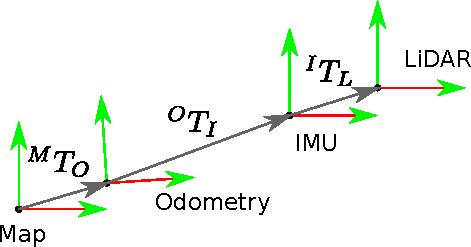
\includegraphics[width=0.4\textwidth]{../figs/frames.pdf}
  \caption{Coordinate frames employed in this work.}
  \label{fig:frames}
\end{figure}

本書で扱う座標系は主に図\ref{fig:frames}に示すように地図,オドメトリ,IMU,LiDARの4つの座標になります.
それぞれの座標は,$M$,$O$,$I$,$L$の添字により表すこととします.
例えばある点${\bf p}$がそれぞれの座標で定められる場合,左上に添え字を置きそれぞれ${}^{M}{\bf p}$,${}^{O}{\bf p}$,${}^{I}{\bf p}$,${}^{L}{\bf p}$と表します.
またある点の座標変換(Source $S$からTarget $T$への変換)を考えるとき,以下のどちらかを用いて表します.
%
\begin{align}
  \begin{gathered}
    {}^{T}{\bf p} = {}^{T}R_{S} {}^{S}{\bf p} + {}^{T}{\bf t}_{S} \\
%
    {}^{T}{\bf p} = {}^{T}T_{S} {}^{S}{\bf p}
  \end{gathered}
  \label{eq:point_transformation}
\end{align}
%
ただし${\rm SE}(3)$を用いるときは${\bf p} \in \mathbb{R}^{4}$となり,4要素目には1が入ることになります.

例えば,IMU座標からオドメトリ座標に点を変換する場合は,${}^{O}{\bf p} = {}^{O}R_{I} {}^{I}{\bf p} + {}^{O}{\bf t}_{I}$,もしくは${}^{O}{\bf p} = {}^{O}T_{I} {}^{I}{\bf p}$と表記します.
また,もしIMU座標から地図座標への変換を直接考えるときは,以下のどちらかを用います.
%
\begin{align}
  \begin{gathered}
    {}^{M}{\bf p} = {}^{M}R_{O} \left( {}^{O}R_{I} {}^{I}{\bf p} + {}^{O}{\bf t}_{I} \right) + {}^{M}{\bf t}_{O}\\
%
    {}^{M}{\bf p} = {}^{M}T_{O} {}^{O}T_{I} {}^{I}{\bf p}
  \end{gathered}
  \label{eq:point_transformation_synthesis}
\end{align}
%
ただし,${}^{M}T_{I} = {}^{M}T_{O} {}^{O}T_{I}$とし,またこれに対応する並進ベクトルと回転行列を${}^{M}{\bf t}_{I}$,${}^{M}R_{I}$とすれば,式(\ref{eq:point_transformation_synthesis})は式(\ref{eq:point_transformation})のように1つの変換にまとめて書くこともできます.

なお図\ref{fig:frames}に示すそれぞれの座標変換ですが,基本的には,IMUとLiDAR間の変換${}^{I}T_{L}$は静的であるため事前にキャリブレーションで求め,LIOが${}^{O}T_{I}$,SLAM(もしくは自己位置推定)が${}^{M}T_{O}$を求めることになります.
ただし,${}^{I}T_{L}$もオンラインで最適化することもできます.
またSLAMや自己位置推定を使わずに,LIOが直接地図座標への変換を求めると仮定する場合もあるため,図\ref{fig:frames}に示す座標を必ず守らなければならないということではありません.



\chapter{Scan Matching}
\label{sec:scan_matching}

\section{Overview of Scan Matching}

Scan matching refers to the process of finding a rigid transformation $T = \left( R \mid {\bf t} \right) \in {\rm SE}(3)$ that correctly aligns two point clouds.
Suppose we consider aligning two point clouds, $\mathcal{P} = ({\bf p}_{1}, \cdots, {\bf p}_{N})$ and $\mathcal{Q} = ({\bf q}_{1}, \cdots, {\bf q}_{M})$, where ${\bf p}, {\bf q} \in \mathbb{R}^{3}$.
In this case, we consider the following cost function\footnote{In implementation, the Huber loss shown in equation~(\ref{eq:huber_loss}) is employed. However, to avoid unnecessary complexity in the explanation, the Huber loss is omitted in this chapter.}.
%
\begin{align}
  E({\bf t}, R) = \sum_{i=1}^{N} \left\| {\bf q}_{i} - \left( R {\bf p}_{i} + {\bf t} \right) \right\|_{2}^{2},
  \label{eq:icp_cost_SO(3)}
\end{align}
%
where ${\bf q}_{i}$ denotes the point in $\mathcal{Q}$ that is closest to the transformed point $R {\bf p}_{i} + {\bf t}$.
To search for such nearest neighbors, data structures such as kd-trees are typically used.
In the implementation presented in this book, we employ the library {\it nanoflann}\footnote{\url{https://github.com/jlblancoc/nanoflann}}.

Equation~(\ref{eq:icp_cost_SO(3)}) can also be written as follows.
%
\begin{align}
  E(T) = \sum_{i=1}^{N} \left\| {\bf q}_{i} - T {\bf p}_{i} \right\|_{2}^{2}.
  \label{eq:icp_cost_SE(3)}
\end{align}
%
When expressed in the form of equation~(\ref{eq:icp_cost_SE(3)}), we have ${\bf p}, {\bf q} \in \mathbb{R}^{4}$, with the fourth element of each set to $1$.
Consequently, $T{\bf p}$ is also a four-dimensional vector with its fourth element equal to $1$.
Since the fourth element of ${\bf q}$ is likewise $1$, the fourth component of ${\bf q} - T{\bf p}$ is always zero.
As a result, the value of the cost function is identical to that given in equation~(\ref{eq:icp_cost_SO(3)}).
In the following, we define ${\bf r} = {\bf q} - T{\bf p}$ as the residual vector.

In scan matching, the goal is to estimate the rigid transformation shown below.
%
\begin{align}
  T^{*} = \argmin_{T} E(T).
  \label{eq:icp_scan_matching}
\end{align}
%
Equation~(\ref{eq:icp_scan_matching}) indicates that the goal is to find the pose $T^{*}$ that minimizes the cost function $E$.
Since $T^{*}$ is generally obtained through an iterative process, this method is referred to as {\bf Iterative Closest Point} (ICP) scan matching.
Note that scan matching that minimizes the cost defined in equation~(\ref{eq:icp_cost_SE(3)}) seeks to minimize the distances between corresponding points, and is therefore called point-to-point ICP.

However, point-to-point ICP is generally considered sensitive to noise.
For this reason, in this book we focus on point-to-plane ICP, which minimizes the distance between points and planes and is known to provide greater robustness.
In point-to-plane ICP, the following cost function is considered.
%
\begin{align}
  E(T) = \sum_{i=1}^{N} \left( {\bf n}_{i}^{\top} {\bf r}_{i} \right)^{2},
  \label{eq:point-to-plane_icp_cost_SE(3)}
\end{align}
%
where ${\bf n}_{i}$ denotes the normal vector in three-dimensional space, computed from the neighboring points of ${\bf q}_{i}$, and we define the residual as $r_{i} = {\bf n}_{i}^{\top} {\bf r}_{i}$.
These relationships are illustrated in Fig.~\ref{fig:normal_residual}.
Note that since ${\bf r}$ is a four-dimensional vector, ${\bf n}$ is also expressed as a four-dimensional vector.
However, because the fourth component of ${\bf r}$ is always zero, the value of the fourth component of ${\bf n}$ has no effect on the computation.

\begin{figure}[!t]
  \centering
  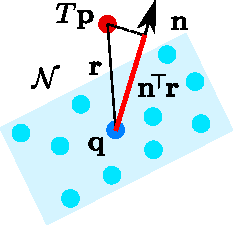
\includegraphics[width=0.2\textwidth]{../figs/normal_residual.pdf}
  \caption{Residual error used in point-to-plane ICP.}
  \label{fig:normal_residual}
\end{figure}

In the following, we first describe the method for computing the normal vectors, then derive the Jacobian associated with the residual vector, and finally explain how this Jacobian is used to perform optimization via the Gauss-Newton method.










\section{Computation of Normal Vectors}

To compute the normal vector at a point ${\bf q}$, we first collect the neighboring points around ${\bf q}$ and denote this set as $\mathcal{N}$.
Using this set, we then compute the mean $\bar{{\bf q}}$.
%
\begin{align}
  \bar{ {\bf q} } = \frac{1}{ | \mathcal{N} | } \sum_{ {\bf q}_{i} \in \mathcal{N} } {\bf q}_{i}.
  \label{eq:points_mean}
\end{align}
%
Next, we compute the covariance matrix $C$ of $\mathcal{N}$.
%
\begin{align}
  C = \frac{1}{ | \mathcal{N} | } \sum_{ {\bf q}_{i} \in \mathcal{N} } \left( {\bf q}_{i} - \bar{ {\bf q} } \right) \left( {\bf q}_{i} - \bar{ {\bf q} } \right)^{\top}.
  \label{eq:points_covariance}
\end{align}
%
Then, we perform eigen decomposition of $C$.
%
\begin{align}
  C = V \Lambda V^{\top},
\end{align}
%
where $V = \left( {\bf v}_{1} ~ {\bf v}_{2} ~ {\bf v}_{3} \right)$ and $\Lambda = {\rm diag} \left( \lambda_{1}, \lambda_{2}, \lambda_{3} \right)$, where ${\bf v}_{i}$ and $\lambda_{i}$ denote the eigenvectors and their corresponding eigenvalues, respectively.

The eigenvalues represent the variance of the points along each direction.
The eigenvector corresponding to the smallest eigenvalue indicates the direction with the least variance, i.e., the most compressed direction.
Therefore, when the smallest eigenvalue $\lambda_{\min}$ is sufficiently small, the corresponding eigenvector ${\bf v}_{\min}$ can be regarded as the normal vector of the local plane on which the points lie.
The vector ${\bf v}_{\min}$ obtained in this way is defined as the normal vector ${\bf n}$ at point ${\bf q}$.
Moreover, by setting a threshold on $\lambda_{\min}$, points with insufficient planarity can be excluded.










\section{Computation of the Jacobian}
\label{subsec:point_to_plane_jacobian}

In solving point-to-plane ICP using the Gauss-Newton method, we derive the Jacobian of the residual $r = {\bf n}^{\top} {\bf r}$ with respect to the pose $T$.
This Jacobian can be computed using the chain rule as follows.
%
\begin{align}
  \frac{ \partial r }{ \partial T } = \frac{ \partial r }{ \partial {\bf r} }
                                      \frac{ \partial {\bf r} }{ \partial T }.
\end{align}
%
Since $r = {\bf n}^{\top} {\bf r}$, it is clear that $\partial r / \partial {\bf r} = {\bf n}^{\top}$.
Therefore, in the following, we present the detailed computation only for $\partial {\bf r} / \partial T$.

The residual vector ${\bf r}$ is clearly a function of the pose $T$.
Thus, the Jacobian $J$ can be derived by considering the following expression.
%
\begin{align}
  {\bf r} \left( \exp \left( \delta \boldsymbol \xi^{\wedge} \right) T \right) - {\bf r} \left( T \right) =
  J \delta \boldsymbol \xi,
  \label{eq:point_plane_icp_jacob_approx}
\end{align}
%
where $\delta \boldsymbol{\xi}^{\wedge} = \left( \delta {\bf v}^{\top} ~ \delta \boldsymbol{\phi}^{\top} \right)^{\wedge} \in \mathfrak{se}(3)$, and $\exp \left( \delta \boldsymbol{\xi}^{\wedge} \right) T$ represents the state obtained by applying an infinitesimal perturbation to $T$ from the left in the space of ${\rm SE}(3)$.
Expanding the left-hand side of equation~(\ref{eq:point_plane_icp_jacob_approx}) yields the following.
%
\begin{align}
  \begin{split}
    {\bf q} - \exp \left( \delta \boldsymbol \xi^{\wedge} \right) T {\bf p} - \left( {\bf q} - T {\bf p} \right)
    %
    = & - \left( \exp \left( \delta \boldsymbol \xi^{\wedge} \right) - I_{4} \right) T {\bf p}, \\
    %
    = & - \left( \left( \begin{matrix} I_{3} + \delta \boldsymbol \phi^{\wedge} & \delta {\bf v} \\ {\bf 0}^{\top} & 1 \end{matrix} \right) - I_{4} \right) \left( \begin{matrix} R {\bf p} + {\bf t} \\ 1 \end{matrix} \right), \\
    %
    = & - \left( \begin{matrix} \delta \boldsymbol \phi^{\wedge} & \delta {\bf v} \\ {\bf 0}^{\top} & 0 \end{matrix} \right) \left( \begin{matrix} {\bf p}^{'} \\ 1 \end{matrix} \right), \\
    %
     = & - \left( \begin{matrix} \delta \boldsymbol \phi^{\wedge} {\bf p}^{'} + \delta {\bf v} \\ 0 \end{matrix} \right), \\
    %
     = & \left( \begin{matrix} \left( {\bf p}^{'} \right)^{\wedge} \delta \boldsymbol \phi - \delta {\bf v} \\ 0 \end{matrix} \right), \\
     %
     = & \left( \begin{matrix} -I_{3} & \left( {\bf p}^{'} \right)^{\wedge} \\ {\bf 0}^{\top} & {\bf 0}^{\top} \end{matrix} \right) \delta \boldsymbol \xi,
  \end{split}
\end{align}
%
where we set ${\bf p}^{'} = R{\bf p} + {\bf t}$ and use the relation $\delta \boldsymbol{\phi}^{\wedge} {\bf p}^{'} = -\left( {\bf p}^{'} \right)^{\wedge} \delta \boldsymbol{\phi}$.
Therefore, the Jacobian with respect to the residual is given as follows.
%
\begin{align}
  \begin{split}
    \frac{ \partial r }{ \partial T } = & {\bf n}^{\top} \left( \begin{matrix} -I_{3} & \left( {\bf p}^{'} \right)^{\wedge} \\ {\bf 0}^{\top} & {\bf 0}^{\top} \end{matrix} \right), \\
    %
    = & \left( \begin{matrix} -{\bf n}^{\top} & {\bf n}^{\top} \left( {\bf p}^{'} \right)^{\wedge} \end{matrix} \right) \in \mathbb{R}^{1 \times 6}.
  \end{split}
  \label{eq:point_to_plane_icp_jacobian}
\end{align}
%
Note that the final ${\bf n} \in \mathbb{R}^{3}$ represents the three-dimensional normal vector.













\section{Optimization Using the Gauss-Newton Method}

Using the Jacobian given in equation~(\ref{eq:point_to_plane_icp_jacobian}), the Hessian matrix and gradient vector for solving point-to-plane ICP scan matching with the Gauss-Newton method are obtained as follows.
%
\begin{align}
  \begin{gathered}
    H = \sum_{i=1}^{N} J_{i}^{\top} J_{i}, \\
    {\bf b} = \sum_{i=1}^{N} J_{i}^{\top} r_{i}. 
  \end{gathered}
  \label{eq:point_to_plane_icp_hessian_and_gradient}
\end{align}
%
When using the Huber loss, we define $w_{i} = \rho^{\prime}\left( r_{i}^{2} \right)$ based on equation~(\ref{eq:huber_loss_prime}), and compute $H = \sum_{i} w_{i} J_{i}^{\top} J_{i}$ and ${\bf b} = \sum_{i} w_{i} J_{i}^{\top} r_{i}$.
Then, using $H$ and ${\bf b}$ as defined in equation~(\ref{eq:point_to_plane_icp_hessian_and_gradient}), we solve for $\delta \boldsymbol{\xi}$ such that $H \delta \boldsymbol{\xi} = -{\bf b}$.
Finally, the state is updated as follows.
%
\begin{align}
  T \leftarrow \exp \left( \delta \boldsymbol \xi^{\wedge} \right) T.
\end{align}
%
This update is repeated until either $\| \delta \boldsymbol{\xi} \|_{2} \leq \epsilon$ or a predefined number of iterations is reached, at which point $T^{*}$ in equation~(\ref{eq:icp_scan_matching}) is considered to have been obtained.
Here, $\epsilon$ is an arbitrary constant.












\section{Practical Considerations}
\label{sec:scan_matching_実用にあたって}

To execute scan matching accurately, obtaining a good initial estimate is of critical importance.
If the initial estimate is sufficiently accurate, correspondence search operates reliably, and scan matching converges to the optimal solution with high precision.
Conversely, if the initial estimate contains large errors, correspondence search is likely to fail, causing scan matching to break down.
It should also be noted that scan matching may converge to a solution that does not minimize the cost function; such solutions are referred to as {\bf local minima}.

To mitigate the effects of incorrect correspondences, it is effective to introduce a robust kernel such as the Huber loss.
By suppressing the influence of large residuals, the Huber loss can prevent optimization from being significantly degraded by outliers.
However, the Huber loss is not a universal remedy.
For instance, when a small number of correct correspondences are mixed with a large number of incorrect ones, the residuals of the correct correspondences may still be large.
In such cases, the Huber loss reduces their weights as well, leading to an underestimation of their contribution.
As a result, scan matching may succeed without the Huber loss but fail when it is applied.
Therefore, the parameter $\delta$ of the Huber loss must be carefully tuned.
Nevertheless, in most cases, introducing the Huber loss improves the robustness of scan matching.

It is also difficult for scan matching alone to provide a reliable initial estimate at every frame, particularly when the motion involves high translation or rotation speeds.
To address this issue, it is effective to integrate external sensors such as IMUs, which can provide more accurate initial estimates.
In the next chapter, we discuss a method for loosely coupling LiDAR and IMU measurements.

In addition to the initial estimate, attention must also be paid to the environment in which scan matching is performed.
Since scan matching determines rigid transformations based on geometric constraints, obtaining the correct solution requires an environment that provides sufficient constraints.
If appropriate constraints cannot be obtained, solving the Gauss-Newton equations $H \delta \boldsymbol{\xi} = -{\bf b}$ may fail to yield a valid $\delta \boldsymbol{\xi}$.
This occurs because $H$ becomes non-invertible, and its inverse cannot be defined.
Such cases are referred to as {\bf degeneracy}, in which scan matching fundamentally fails to function.
A common method to detect degeneracy is to perform eigenvalue decomposition of the Hessian matrix defined in equation~(\ref{eq:point_to_plane_icp_hessian_and_gradient}) and examine its smallest eigenvalue.
If the smallest eigenvalue is extremely small, the Hessian matrix becomes rank-deficient, preventing computation of a valid inverse.
Consequently, the optimization process breaks down.



\chapter{ルーズカップリングに基づくLIO}
\label{sec:loose_coupling_lio}

\section{状態量と問題設定}
\label{eq:state_and_problem_setting_loose_coupling}

前章で述べたスキャンマッチングでは,姿勢$T \in {\rm SE}(3)$のみを求める問題を考えていました.
これに対して本章で述べるLIOでは,以下の状態量を求めることを考えます.
%
\begin{align}
  {\bf x} = \left( {}^{O}{\bf t}_{I} ~ {}^{O}R_{I} ~ {}^{O}{\bf v} ~ {\bf b}^{\omega} ~ {\bf b}^{a} \right)
  \label{eq:loose_coupling_lio_state}
\end{align}
%
ここで${}^{O}{\bf t}_{I} \in \mathbb{R}^{3}$と${}^{O}R_{I} \in {\rm SO}(3)$は,オドメトリ座標でのIMUの姿勢を表す並進ベクトルと回転行列,${}^{O}{\bf v} \in \mathbb{R}^{3}$はオドメトリ座標系におけるIMUの速度ベクトル,${\bf b}^{\omega}, {\bf b}^{a} \in \mathbb{R}^{3}$はIMUの角速度と加速度に対するバイアスになります.
なお,$\left( \log \left( R \right) \right)^{\vee} \in \mathbb{R}^{3}$となるので,本章で述べるLIOでは15次元の状態を推定する問題となります.
また,IMUの姿勢を求めていることに注意してください.

LIOではLiDARとIMUを用いるため,各センサデータの時間軸を考えることが重要になります.
例えばLiDARが時刻$t-1$および$t$において,それぞれ$\mathcal{P}_{t-1}$,$\mathcal{P}_{t}$の点群を取得するとします.
この間,IMUは$\mathcal{U}_{t} = \left( \boldsymbol \omega_{t}^{1} ~ {\bf a}_{t}^{1} ~ \cdots ~ \boldsymbol \omega_{t}^{M_{t}} ~ {\bf a}_{t}^{M_{t}} \right)$のデータを計測するとします\footnote{一般にIMUの方がLiDARより計測周期が高いため,LiDARが計測を行う間にIMUの計測値は複数個存在します.}.
なお図\ref{fig:time_relationships}に,これらのセンサデータ,および本章で使われる時間の関係を図示しています.

本章で解説するLIOでは,LiDARとIMUの計測値を用いて,式(\ref{eq:loose_coupling_lio_state})に示す状態量を求めることが目標になり,これは以下の処理を繰り返すことで達成されます.
%
\begin{enumerate}
  \item IMUプレインテグレーションを用いた状態の予測
  \item LiDAR点群の歪み補正
  \item 局所地図とLiDAR点群のスキャンマッチング
  \item 予測およびスキャンマッチングの結果に基づく状態の再更新
  \item キーフレームの検出と局所地図の構築
\end{enumerate}
%
なお4の再更新の部分がルーズカップリングに相当し,これにはDirectLIO~\cite{DirectLIO}で用いられているHierarchical Geometric Observer(HGO)\cite{Lopez2023arXiv}を用います.
ただしHGOの利用がルーズカップリングとして良い方法であるということではなく,実装が用意なので紹介しているということに留意ください.
実装できるなら,拡張カルマンフィルたのような実装をするほうが良いといえます.

\begin{figure}[!t]
  \centering
  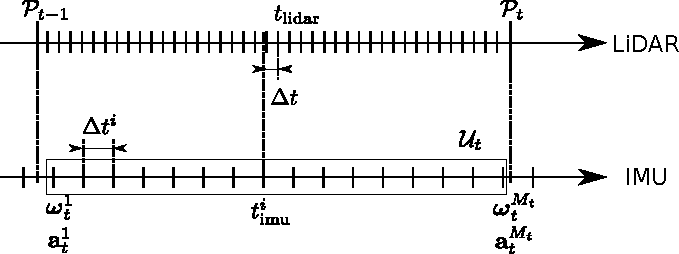
\includegraphics[width=0.6\textwidth]{../figs/time_relationships.pdf}
  \caption{Temporal relationship between LiDAR and IMU measurements.}
  \label{fig:time_relationships}
\end{figure}
















\section{IMUプレインテグレーション}
\label{subsec:imu_preintegration}

今時刻$t-1$の状態${\bf x}_{t-1}$まで推定が行われていて,時刻$t$のIMUのデータ$\mathcal{U}_{t}$が得られているとします.
スキャンマッチングを実行するにあたり,{\bf IMUプレインテグレーション}(IMU Preitegration)を用いて,回転行列,並進ベクトル,および速度ベクトルを以下のように更新します.
%
\begin{align}
  \begin{gathered}
    {}^{O}{\bf t}_{I, t} = {}^{O}{\bf t}_{I, t-1} + \sum_{i=1}^{M_{t}} {}^{O}{\bf v}_{t-1}^{j} \Delta t^{i} + \frac{1}{2} {}^{O}R_{I, t-1}^{j} \left( {\bf a}_{t}^{i} - {\bf b}_{t-1}^{a} \right) \left( \Delta t^{i} \right)^{2} + \frac{1}{2} {\bf g} \left( \Delta t^{i} \right)^{2} \\
%
    {}^{O}R_{I, t} = {}^{O}R_{I, t-1} \prod_{i=1}^{M_{t}} \exp \left( \left( \boldsymbol \omega_{t}^{i} - {\bf b}_{t-1}^{\omega} \right)^{\wedge} \Delta t^{i} \right) \\
%
    {}^{O}{\bf v}_{t} = {}^{O}{\bf v}_{t-1} + \sum_{i=1}^{M_{t}} {}^{O}R_{I, t-1}^{j} \left( {\bf a}_{t}^{i} - {\bf b}_{t-1}^{a} \right) \Delta t^{i} + {\bf g} \Delta t^{i} \\
  \end{gathered}
  \label{eq:discrete_imu_preintegration}
\end{align}
%
ここで${\bf g}$は重力加速度ベクトル,$\Delta t^{i}$は$i$番目から$i-1$番目のIMUの計測時間の差,${}^{O}R_{I, t-1}^{j}$と${}^{O}{\bf v}_{I, t-1}^{j}$はそれぞれ以下となります.
\begin{align}
  \begin{gathered}
    {}^{O}R_{I, t-1}^{j} = {}^{O}R_{I, t-1} \prod_{i=1}^{j} \exp \left( \left( \boldsymbol \omega_{t}^{i} - {\bf b}_{t-1}^{\omega} \right)^{\wedge} \Delta t^{i} \right) \\
%
    {}^{O}{\bf v}_{t-1}^{j} = {}^{O}{\bf v}_{t-1} + \sum_{i=1}^{j} {}^{O}R_{I, t-1}^{j} \left( {\bf a}_{t}^{i} - {\bf b}_{t-1}^{a} \right) \Delta t^{i} + {\bf g} \Delta t^{i} \\
  \end{gathered}
\end{align}
%
次に示すスキャンマッチングでは,式(\ref{eq:discrete_imu_preintegration})に示す並進ベクトルと回転行列を初期値として用います.
















\section{歪み補正}
\label{subsec:deskew_scan_distortion}

一般的にIMUの計測周期はLiDARの計測周期より高いです.
そのため,LiDARが1周期分の点群を計測する間に,複数のIMUの計測値を取得することが可能です.
そしてこの計測値を利用すると,式(\ref{eq:discrete_imu_preintegration})に示すように,LiDARが1周期分の点群を取得する間の姿勢を計算することができます.
そしてこれらの姿勢を利用すると,LiDARが計測した各点をより正確な位置に補正することができます.
この操作を,LiDARのデータの歪み補正と呼びます.

歪み補正の解説を行う前に,まずIMUプレインテグレーションにより得られた$M_{t}+1$個の姿勢の集合を$\left( {}^{O}T_{I}^{0}, \cdots, {}^{O}T_{I}^{M_{t}} \right)$とし,またこれらの姿勢列に対応した$M_{t}+1$個の時間の集合を$\left( t_{\rm imu}^{0}, \cdots, t_{\rm imu}^{M_{t}} \right)$とします.
なお,${}^{O}T_{I}^{j} = \left( {}^{O}R_{I, t-1}^{j} \mid {}^{O}{\bf t}_{I, t-1}^{j} \right) \in {\rm SE}(3)$です.
また,${}^{O}T_{I}^{0} = {}^{O}T_{I, t-1}$,${}^{O}T_{I}^{M_{t}} = {}^{O}T_{I, t}$となります.

歪み補正を行う前提として,LiDARが計測した各点にタイムスタンプが付与されていることを前提とします.
そしてこのタイムスタンプを用いて,$t_{\rm imu}^{i} \leq t_{\rm lidar} \leq t_{\rm imu}^{i+1} ~ \left( i = 0, \cdots, M_{t}-1 \right)$となるIMUの計測値を探索します.
今,$i$番目と$i+1$番目の時間の間でLiDARが点${}^{L}{\bf p}$を計測していたとします.
このとき,この点を計測した際のIMUの姿勢を以下のように求めます.
%
\begin{align}
  \begin{gathered}
    \Delta t = t_{\rm lidar} - t_{\rm imu}^{i} \\
%
    {}^{O}R_{I}^{d} = {}^{O}R_{I, t-1}^{i} \exp \left( \left( \boldsymbol \omega_{t}^{i} - {\bf b}_{t-1}^{\omega} 
\right)^{\wedge} \Delta t \right) \\
%
    {}^{O}{\bf t}_{I}^{d} = {}^{O}{\bf t}_{I, t-1}^{i} + {}^{O}{\bf v}_{t-1}^{i} \Delta t + \frac{1}{2} {}^{O}R_{I, t-1}^{i} \left( {\bf a}_{t}^{i} - {\bf b}_{t-1}^{a} \right) \Delta t^{2} + \frac{1}{2} {\bf g} \Delta t^{2}
  \end{gathered}
\end{align}
%
そして,${}^{O}T_{I}^{d} = \left( {}^{O}R_{I}^{d} \mid {}^{O}{\bf t}_{I}^{d} \right)$を定め,${}^{L}{\bf p}$を以下のようにIMU座標の点に変換します.
%
\begin{align}
  {}^{I}{\bf p} = \left( {}^{O}T_{I}^{M_{t}} \right)^{-1} {}^{O}T_{I}^{d} {}^{I}T_{L} {}^{L}{\bf p}
\end{align}
%
ここで${}^{I}T_{L}$はLiDARとIMU間の剛体変換を表す行列であり,事前に求められているものとしています.
この操作をすべての計測点群に対して行うことで,LiDARが計測した点群の歪みを補正することができます.
なお一番最後に$\left( {}^{O}T_{I}^{M_{t}} \right)^{-1}$を適用することで,式(\ref{eq:discrete_imu_preintegration})で予測したIMUの姿勢を原点とした座標の点群が得られます.


















\section{局所地図とのスキャンマッチング}

IMUプレインテグレーションによる予測,および歪み補正を終えた後に,{\bf 局所地図}(Local Map)とのスキャンマッチングを実施します.
なお説明の都合上先に局所地図とのスキャンマッチングについて述べますが,局所地図の作成方法に関しては\ref{subsec:local_map_building}節で述べます.
またスキャンマッチングに関しては基本的に\ref{sec:scan_matching}章で述べた方法を用いますが,本節では使用されるデータや座標に関して整理しておきます.

まず局所地図を表す点群${}^{O}\mathcal{M}$が,オドメトリ座標上で構築されているとします\footnote{局所座標の構築方法にも様々な方法があり,明示的にオドメトリ座標で地図構築を行わない方法もあります.}.
また前節で述べた歪み補正も適用され,LiDARの計測点群はIMU座標での点群${}^{I}\mathcal{P}$が得られているとします.
このとき,LiDARの計測点${}^{I}{\bf p}$に対する残差ベクトルを以下のように定めます.
%
\begin{align}
  {\bf r} = {}^{O}{\bf q} - {}^{O}T_{I} {}^{I}{\bf p}
  \label{eq:residual_vector_lio_scan_matching}
\end{align}
%
なお${}^{O}{\bf q}$は,${}^{O}\mathcal{M}$の点で${}^{O}T_{I} {}^{I}{\bf p}$に最も近い点です.
そして,以下に示すコスト関数の最小化を行います.
%
\begin{align}
  E \left( {}^{O}T_{I} \right) = \sum_{i=1}^{N} \rho \left( \left\| {\bf n}_{i}^{\top} {\bf r}_{i} \right\|_{2}^{2} \right)
  \label{eq:cost_function_lio_scan_matching}
\end{align}
%
ただし${\bf n}$は,${}^{O}{\bf q}$に対応する法線ベクトルになります.















\section{ルーズカップリングによる状態量の更新}

IMUプレインテグレーションにより予測された姿勢を${}^{O}\hat{T}_{I}$,スキャンマッチングにより得られた姿勢を${}^{O}T_{I}^{*}$とします.
またこれらに対応する並進ベクトルと回転行列に対応するクォータニオンをそれぞれ${}^{O}\hat{ {\bf t} }_{I}$,${}^{O}{\bf t}_{I}^{*}$,${}^{O}\hat{ {\bf q} }_{I}$,${}^{O}{\bf q}_{I}^{*}$とします.
これらを用いて,最新の状態をそれぞれ以下のように更新します.
%
\begin{align}
  \begin{gathered}
    {}^{O}{\bf q}_{I} = {}^{O}\hat{ {\bf q} }_{I} + \Delta t \gamma_{1} {}^{O}\hat{ {\bf q} }_{I} \left( \begin{matrix} 1 - \left| q_{w}^{d} \right| \\ {\rm sgn} \left( q_{w}^{d} \right) {\bf q}_{v}^{d} \end{matrix} \right) \\
    {\bf b}^{\omega} = \hat{ {\bf b} }^{\omega} - \Delta t \gamma_{2} q_{w}^{d} {\bf q}_{v}^{d} \\
    {}^{O}{\bf t}_{I} = {}^{O}\hat{ {\bf t} }_{I} + \Delta t \gamma_{3} {\bf t}^{d} \\
    {}^{O}{\bf v} = {}^{O}\hat{ {\bf v} }_{t} + \Delta t \gamma_{4} {\bf t}^{d} \\
    {\bf b}^{a} = \hat{ {\bf b} }^{a} - \Delta t \gamma_{5} {}^{O}\hat{R}_{I}^{\top} {\bf t}^{d}
  \end{gathered}
\end{align}
%
ここで$\Delta t$はIMUプレインテグレーションを行った時間の総和,$\gamma_{1-5}$は任意の正の定数,${\bf q}^{d} = {}^{O}\hat{ {\bf q} }_{I}^{-1} \otimes {}^{O}{\bf q}_{I}^{*}$,${\bf t}^{d} = {}^{O}{\bf t}_{I}^{*} - {}^{O}\hat{ {\bf t} }_{I}$です.
また${\bf q}^{d} = \left( q_{w}^{d} ~ \left( {\bf q}_{v}^{d} \right)^{\top} \right)^{\top}$,${\bf q}_{v}^{d} = \left( q_{x}^{d} ~ q_{y}^{d} ~ q_{z}^{d} \right)^{\top}$であり,${}^{O}\hat{R}_{I}$は${}^{O}\hat{ {\bf q} }_{I}$に対応する回転行列です.



















\section{局所地図の構築}
\label{subsec:local_map_building}

局所地図を構築する方法も様々ありますが,本書ではキーフレームを用いた方法を採用します.
具体的には,LIOが推定する姿勢の中からいくつかの姿勢をキーフレームとして選択し,その姿勢とそれに対応するLiDARの点群を用いて局所地図${}^{O}\mathcal{M}$の作成を行います.
キーフレームの検出にあたっては,最も単純な方法ではありますが,移動量に対して閾値を設け,前回検出したキーフレームからの並進移動量,もしくは回転量が一定値を超えた場合に,新たにキーフレームとして検出を行います.

今キーフレームの集合として$\left( {}^{O}T_{I, 1}, \cdots, {}^{O}T_{I, K} \right)$,またこれらのキーフレームに対応したLiDARの点群$\left( {}^{I}\mathcal{P}_{1}, \cdots, {}^{I}\mathcal{P}_{K} \right)$があるとします.
なお$K$は局所地図を構築するために使用するキーフレームの数です.
これらの点すべてを対応するキーフレームでオドメトリ座標に変換した点の集合を局所地図として定めます.
%
\begin{align}
  {}^{O}\mathcal{M} = \bigcup_{i=1}^{K} \bigcup_{{}^{I}{\bf p} \in {}^{I}\mathcal{P}_{i}} {}^{O}T_{I, i} {}^{I}{\bf p}
\end{align}
%

キーフレームをいくつ利用するかにもよりますが,通常局所地図は大きな点群となります.
そのため,すべての点に対して法線ベクトルを計算すると非常に大きな計算コストが発生します.
また局所地図が大きくなると,スキャンマッチングに使用されない点も多く含まれてきます.
そのため本実装では,式(\ref{eq:residual_vector_lio_scan_matching})に示す残差ベクトルが定義されたときに,その点に対応する法線ベクトルの計算を行うことにします.
また,計算済みかどうかを判定するフラグも実装し,局所地図構築に関する計算コストの削減を行っています.















\section{実用にあたって}

ルーズカップリングに基づくLIOは,次章で述べるタイトカップリングに基づくLIOと比較すると,実装やパラメータ調整が容易に行うことができます.
加えて,おおよその環境では十分な性能を持って機能します.
そのため,まずLIOを実装し,LiDARとIMUを融合させる方法を知りたいという方には,適した手法であるといえます.
ただし多くの場合,タイトカップリングに基づくLIOの方が精度が高い傾向にあります.
ただしタイトカップリングに基づくLIOは実装やパラメータ調整の難易度が上がります.
繰り返しにはなりますが,ルーズカップリングに基づくLIOも十分な性能を持つため,ルーズカップリングが良いかタイトカップリングが良いかは,ユーザーの状況次第になるといえます.

LIOで最も計算コストがかかる部分は,局所地図の構築部分になります.
局所地図はサイズを小さくすれば構築の計算コストは下がりますが,その分スキャンマッチングに利用できる範囲が限定されるため,移動量推定においてドリフト誤差が発生しやすくなってしまいます.
しかし局所地図のサイズを大きくしすぎると,地図構築の計算コストが増大し,最悪の場合,LiDARの計測周期を超えるような計算時間となり,LIOの破綻に繋がってしまいます.

また局所地図の更新頻度もLIOの精度に大きく関わります.
特にLiDARの観測がスキャンマッチングに適さないような環境では,できる限り局所地図を更新する頻度を向上させた方がLIOの精度を維持することができます.
しかし当然ながら,局所地図の更新頻度が増えるほど計算コストの増大にも繋がります.
また本実装では,単純な移動量に対して閾値を設けて局所地図の更新をおこなっているため,局所地図の更新頻度を高くすると,局所地図として地図化できる範囲が小さくなり,これもドリフト誤差を発生させやすくなる要因になります.
LIOの精度が低下する場合などは,局所地図に関するパラメータの調整,またもしくは,局所地図の更新ルールを見直すことが効果的なことが多いです.
なおこれらの局所地図に関する問題は,次章で述べるタイトカップリングに基づくLIOでも同様に表れます.




















\chapter{タイトカップリングに基づくLIO}

\section{状態量と問題設定}

前章では,推定対象の状態としてIMUの姿勢(並進ベクトル${}^{O}{\bf t}_{I}$と回転行列${}^{O}R_{I}$),速度${}^{O}{\bf v}$,およびIMUの角速度と加速度に対する計測バイアス${\bf b}^{\omega}$,${\bf b}^{a}$としていました.
タイトカップリングを用いたLIOも同様の状態で実装可能ですが,本章では拡張性を考慮し,状態量を以下とします.
%
\begin{align}
  {\bf x} = \left( {}^{O}{\bf t}_{I} ~ {}^{O}R_{I} ~ {}^{O}{\bf v} ~ {\bf b}^{\omega} ~ {\bf b}^{a} ~ {\bf g} ~ {}^{I}{\bf t}_{L} ~ {}^{I}R_{L} \right)
  \label{eq:tight_coupling_lio_state}
\end{align}
%
ここで${\bf g} \in \mathbb{R}^{3}$は重力加速度ベクトル,${}^{I}{\bf t}_{L} \in \mathbb{R}^{3}$と${}^{I}R_{L} \in {\rm SO}(3)$はLiDARとIMU間の相対姿勢を表す並進ベクトルと回転行列です.
なお,$\left( \log \left( {}^{I}R_{L} \right) \right)^{\vee} \in \mathbb{R}^{3}$となるので,本章で扱うLIOでは24次元の状態推定を行います.
また前章で述べたLIOでは扱いませんでしたが,推定状態に対する共分散行列$\Sigma \in \mathbb{R}^{24 \times 24}$も扱います.













\section{IMUプレインテグレーションによる更新}

本章で述べるLIOでも,\ref{subsec:imu_preintegration}節で述べたIMUプレインテグレーションを用いて,IMUの姿勢と速度の更新を行います.
ただし本章で述べるLIOでは,これらに加えて共分散行列の更新も行います.

共分散行列の更新を考えるにあたり,まずホワイトノイズベクトル$\boldsymbol \eta = \left( \boldsymbol \eta^{\omega} ~ \boldsymbol \eta^{a} ~ \boldsymbol \eta^{ b^{\omega} } ~ \boldsymbol \eta^{ b^{a} } \right)^{\top} \in \mathbb{R}^{12}$を導入します.
なお$\boldsymbol \eta^{\omega}, \boldsymbol \eta^{a}, \boldsymbol \eta^{ b^{\omega} }, \boldsymbol \eta^{ b^{a} } \in \mathbb{R}^{3}$はそれぞれIMUの角速度と加速度の計測値,およびそれらの計測バイアスに加わるホワイトノイズとします.
今,${\bf u}_{t} = \left( \boldsymbol \omega_{t}^{\top} ~ {\bf a}_{t}^{\top} \right)^{\top} \in \mathbb{R}^{6}$として,1つのIMUの計測値に対する更新則を考えます.
これらの条件を用いると,IMUプレインテグレーションに基づく状態の更新は以下のように定めることができます.
%
\begin{align}
  \begin{gathered}
    {}^{O}{\bf t}_{I, t} = {}^{O}{\bf t}_{I, t-1} + {}^{O}{\bf v}_{t-1} \Delta t + \frac{1}{2} {}^{O}R_{I, t-1} \left( {\bf a}_{t} - {\bf b}_{t-1}^{a} - \boldsymbol \eta_{t}^{a} \right)\Delta t^{2} + \frac{1}{2} {\bf g} \Delta t^{2} \\
%
    {}^{O}R_{I, t} = {}^{O}R_{I, t-1} \exp \left( \left( \boldsymbol \omega_{t} - {\bf b}_{t-1}^{\omega} - \boldsymbol \eta_{t}^{\omega} \right)^{\wedge} \Delta t \right) \\
%
    {}^{O}{\bf v}_{t} = {}^{O}{\bf v}_{t-1} + {}^{O}R_{I, t-1} \left( {\bf a}_{t} - {\bf b}_{t-1}^{a} - \boldsymbol \eta_{t}^{a} \right) \Delta t + {\bf g} \Delta t \\
%
    {\bf b}_{t}^{\omega} = {\bf b}_{t-1}^{\omega} + \boldsymbol \eta_{t}^{ b^{\omega} } \Delta t \\
%
    {\bf b}_{t}^{\omega} = {\bf b}_{t-1}^{a} + \boldsymbol \eta_{t}^{ b^{a} } \Delta t \\
%
    {\bf g}_{t} = {\bf g}_{t-1} \\
%
    {}^{I}{\bf t}_{L, t} = {}^{I}{\bf t}_{L, t-1} \\
%
    {}^{I}R_{L, t} = {}^{I}R_{L, t-1}
  \end{gathered}
  \label{eq:discrete_imu_preintegration_tight}
\end{align}
%
ここで$\Delta t$は,IMUの計測にかかった時間です.
%

式(\ref{eq:discrete_imu_preintegration_tight})による状態の更新を${\bf x}_{t} = {\bf f} \left( {\bf x}_{t-1}, {\bf u}_{t}, \boldsymbol \eta_{t} \right)$と記述することとします.
このとき,共分散行列の更新は以下のようにすることで行うことができます.
%
\begin{align}
  \Sigma_{t} = F_{x} \Sigma_{t-1} F_{x}^{\top} + F_{\eta} Q F_{\eta}^{\top}
\end{align}
%
ここで,$F_{x} = \partial {\bf f} / \partial {\bf x}_{t-1} \in \mathbb{R}^{24 \times 24}$,$F_{\eta} = \partial {\bf f} / \partial \boldsymbol \eta_{t} \in \mathbb{R}^{24 \times 12}$となり,$Q \in \mathbb{R}^{12 \times 12}$はプロセスノイズ共分散行列です.
これらは大きな行列なので計算は煩雑になりますが,それぞれ以下のように求めることができます\footnote{何度も計算して確かめてはいますが確実にあっているか自信はありません.}.
%
\begin{align}
  F_{x} = \left( \begin{matrix}
    I_{3} & -A \Delta t^{2} & I_{3} \Delta t & 0 & -\frac{1}{2} {}^{O}R_{I, t-1} \Delta t^{2} & \frac{1}{2} I_{3} \Delta t & 0 & 0 \\
%
    0 & J_{l}^{-1} \left( {}^{O}{\bf r}_{I} \right) {}^{O}R_{I, t}^{\top} & 0 & -J_{l}^{-1} \left( {}^{O}{\bf r}_{I} \right) J_{r} \left( \Delta \boldsymbol \phi_{t} \right) \Delta t & 0 & 0 & 0 & 0 \\
%
    0 & -A \Delta t & I_{3} & 0 & -{}^{O}R_{I, t-1} \Delta t & I_{3} \Delta t & 0 & 0 \\
%
    0 & 0 & 0 & I_{3} & 0 & 0 & 0 & 0 \\
%
    0 & 0 & 0 & 0 & I_{3} & 0 & 0 & 0 \\
%
    0 & 0 & 0 & 0 & 0 & I_{3} & 0 & 0 \\
%
    0 & 0 & 0 & 0 & 0 & 0 & I_{3} & 0 \\
%
    0 & 0 & 0 & 0 & 0 & 0 & 0 & J_{l}^{-1} \left( {}^{I}{\bf r}_{L} \right) \\
  \end{matrix} \right)
  \label{eq:covariance_update_fx}
\end{align}
%
\begin{align}
  F_{\eta} = \left( \begin{matrix}
    0 & -\frac{1}{2} {}^{O}R_{I, t-1} \Delta t^{2} & 0 & 0 \\
%
    -J_{l}^{-1} \left( {}^{O}{\bf r}_{I} \right) J_{r} \left( \Delta \boldsymbol \phi_{t} \right) \Delta t & 0 & 0 & 0 \\
%
    0 & {}^{O}R_{I, t-1} \Delta t & 0 & 0 \\
%
    0 & 0 & I_{3} \Delta t & 0 \\
%
    0 & 0 & 0 & I_{3} \Delta t \\
%
    0 & 0 & 0 & 0 \\
%
    0 & 0 & 0 & 0 \\
%
    0 & 0 & 0 & 0 \\
  \end{matrix} \right)
  \label{eq:covariance_update_feta}
\end{align}
%
なお,$\hat{ \boldsymbol \omega }_{t} = \boldsymbol \omega_{t} - {\bf b}_{t-1}^{\omega} - \boldsymbol \eta_{t}^{\omega}$,$\hat{ {\bf a} }_{t} = {\bf a}_{t} - {\bf b}_{t-1}^{a} - \boldsymbol \eta_{t}^{a}$,$A = \left( {}^{O}R_{I, t-1} \hat{ {\bf a} }_{t} \right)^{\wedge}$,${}^{O}{\bf r}_{I} = \left( \log \left( {}^{O}R_{I, t} \right) \right)^{\vee}$,${}^{I}{\bf r}_{L} = \left( \log \left( {}^{I}R_{L, t} \right) \right)^{\vee}$,$\Delta \boldsymbol \phi_{t} = \hat{ \boldsymbol \omega }_{t} \Delta t$として表記を短縮しています.
また式(\ref{eq:covariance_update_fx}),(\ref{eq:covariance_update_feta})に示す$0$はすべて$\mathbb{R}^{3 \times 3}$の要素がすべて$0$の行列です.











\section{IEKFによる更新}

IMUプレインテグレーションによる更新を終えた後に,\ref{subsec:deskew_scan_distortion}節で述べたLiDAR点群の歪み補正を行います.
そしてLiDARの点群をIMU座標に変換し,式(\ref{eq:residual_vector_lio_scan_matching}),(\ref{eq:cost_function_lio_scan_matching})に示す残差ベクトルとコスト関数を定めます.
そして,残差に対するヤコビアンを求めてコスト関数の最小化を実施しますが,本章で述べるLIOでは,式(\ref{eq:tight_coupling_lio_state})に示す状態を用いて最適化を行うため,求めるヤコビアンは\ref{subsec:point_to_plane_jacobian}節で導出したヤコビアンと異なります.

本章で述べるLIOで求めるヤコビアンは以下となります.
%
\begin{align}
  \frac{ \partial r_{i} }{ \partial {\bf x} }
  = \left(
    \frac{ \partial r_{i} }{ \partial {}^{O}{\bf t}_{I} } ~
    \frac{ \partial r_{i} }{ \partial {}^{O}R_{I} } ~
    \frac{ \partial r_{i} }{ \partial {}^{O}{\bf v} } ~
    \frac{ \partial r_{i} }{ \partial {\bf b}^{\omega} } ~
    \frac{ \partial r_{i} }{ \partial {\bf b}^{a} } ~
    \frac{ \partial r_{i} }{ \partial {\bf g} } ~
    \frac{ \partial r_{i} }{ \partial {}^{I}{\bf t}_{L} } ~
    \frac{ \partial r_{i} }{ \partial {}^{I}R_{L} }
  \right)^{\top} \in \mathbb{R}^{1 \times 24}
  \label{eq:residual_jecobian_tight}
\end{align}
%
それぞれのヤコビアンの導出は省きますが,それぞれ以下となります(角速度ベクトルに関するヤコビアンの導出は\ref{sec:回転および角速度バイアスに関するヤコビアンの導出}節で述べています).
%
\begin{align}
  \begin{gathered}
    \frac{ \partial r_{i} }{ \partial {}^{O}{\bf t}_{I} } = -{\bf n}_{i}^{\top} \\
%
    \frac{ \partial r_{i} }{ \partial {}^{O}R_{I} } = {\bf n}_{i}^{\top} \left( {}^{O}R_{I} {}^{I}{\bf p}_{i} \right)^{\wedge} \\
%
    \frac{ \partial r_{i} }{ \partial {}^{O}{\bf v} } = -\Delta t {\bf n}_{i}^{\top} \\
%
    \frac{ \partial r_{i} }{ \partial {\bf b}^{\omega} } = {\bf n}_{i}^{\top} \left( {}^{O}R_{I} {}^{I}{\bf p}_{i} \right)^{\wedge} J_{r} \left( \Delta \boldsymbol \phi \right) \Delta t \\
%
    \frac{ \partial r_{i} }{ \partial {\bf b}^{a} } = \frac{1}{2} \Delta t^{2} {\bf n}_{i}^{\top} {}^{O}R_{I, t-1} \\
%
    \frac{ \partial r_{i} }{ \partial {\bf g} } = -\frac{1}{2} \Delta t^{2} {\bf n}_{i}^{\top} \\
%
    \frac{ \partial r_{i} }{ \partial {}^{I}{\bf t}_{L} } = {\bf n}_{i}^{\top} {}^{O}R_{I} \\
%
    \frac{ \partial r_{i} }{ \partial {}^{I}R_{L} } = {\bf n}_{i}^{\top} {}^{O}R_{I} \left( {}^{I}R_{L} {}^{L}{\bf p}_{i} \right)^{\wedge} \\
  \end{gathered}
\end{align}
%
ここで${}^{L}{\bf p}$と${}^{I}{\bf p}$は同じ点をLiDAR,およびIMU座標で表したものであり${}^{I}{\bf p} = {}^{I}T_{L} {}^{L}{\bf p}$となります.
また$\Delta \boldsymbol \phi = \left( \boldsymbol \omega_{t} - {\bf b}_{t-1}^{\omega} \right) \Delta t$であり,これは状態量である${\bf b}_{t-1}^{\omega}$が変更される度に再計算します.

残差,およびヤコビアンを求めることができたら,{\bf Iterated Extended Kalman Filter}(IEKF)を用いた更新を行いますが,これは次式に従い状態の反復更新を行うことで達成されます.
%
\begin{align}
  \begin{gathered}
    {\bf r}^{k} = \left( r_{1}^{k} ~ \cdots ~ r_{N}^{k} \right)^{\top} \\
%
    J^{k} = \left( J_{1}^{k} ~ \cdots ~ J_{N}^{k} \right)^{\top} \\
%
    H^{k} = \left( \begin{matrix}
      I_{3} & 0_{3 \times 3} & 0_{3 \times 15} & 0_{3 \times 3} \\
%
      0_{3 \times 3} & J_{l}^{-1} \left( \left( \log \left( \left( {}^{O}R_{I}^{1} \right)^{\top} {}^{O}R_{I}^{k} \right) \right)^{\vee} \right) & 0_{3 \times 15} & 0_{3 \times 3} \\
%
      0_{15 \times 3} & 0_{15 \times 3} & I_{15 \times 15} & 0_{3 \times 3} \\
%
      0_{3 \times 3} & 0_{3 \times 3} & 0_{3 \times 3} & J_{l}^{-1} \left( \left( \log \left( \left( {}^{I}R_{L}^{1} \right)^{\top} {}^{I}R_{L}^{k} \right) \right)^{\vee} \right)
    \end{matrix} \right) \\
%
    \bar{ \Sigma }^{k} = \left( H^{k} \right)^{-1} \Sigma \left( \left( H^{k} \right)^{-1} \right)^{\top} \\
%
    K^{k} = \left( \left( J^{k} \right)^{\top} R^{-1} J^{k} + \left( \bar{ \Sigma }^{k} \right)^{-1} \right)^{-1} \left( J^{k} \right)^{\top} R^{-1} \\
%
    {\bf x}^{k+1} = {\bf x}^{k} \boxplus \left( -K^{k} {\bf r}^{k} - \left( I_{24} - K^{k} J^{k} \right) \left( H^{k} \right)^{-1} \left( {\bf x}^{k} \boxminus {\bf x}^{1} \right) \right)
  \end{gathered}
  \label{eq:iterated_extended_kalman_filter}
\end{align}
%
ここで$R = {\rm diag} \left( \sigma^{2}, \cdots \sigma^{2} \right) \in \mathbb{R}^{N \times N}$であり,$\sigma^{2} \in \mathbb{R}$は残差に対する分散になります.
また,右上に1のつく状態は,反復計算を行う際のそれぞれの初期値になります.
そして,$k$回目の反復計算で更新量が一定以下となり収束したと判定されたら,以下のように状態と共分散行列を更新します.
%
\begin{align}
  \begin{gathered}
    {\bf x}_{t} = {\bf x}^{k} \\
%
    \Sigma_{t} = \left( I_{24} - K^{k} J^{k} \right) \bar{ \Sigma }^{k}
  \end{gathered}
\end{align}























\section{実用にあたって}

前章で述べたルーズカップリングに基づくLIOでは,重力加速度やLiDAR-IMU間の相対姿勢などは推定対象に含まれていませんでした.
一方でタイトカップリングに基づく手法では,これらのパラメータも同時に最適化することが可能です.
これは,ルーズカップリングのように推定を2段階に分ける方法では冗長性が生じるのに対し,タイトカップリングではそのような冗長性を排除し,すべてのパラメータを統一的に推定できるためです.

ただし,これらのパラメータを推定に含めたからといって,常に劇的な性能向上が得られるわけではありません.
しかし多くの場面において,タイトカップリングを用いた方がより高精度な推定結果が得られる傾向があります.
なお,重力加速度やLiDAR-IMU間の相対姿勢を最適化しなくとも,タイトカップリングに基づくLIOは十分に機能するため,これらのパラメータは必ずしも最適化されるべきとは限りません.

本書では扱いませんが,近年ではLiDAR,カメラ,IMUを併用して最適化を行う手法も提案されています.
このような手法においては,LiDAR-カメラ間の相対姿勢を高精度に求めることが極めて重要となります.
しかし,これらの外部パラメータは事前のキャリブレーションのみでは十分に正確に求められないことも多いため,タイトカップリングの枠組みの中でLiDAR-カメラ間の相対姿勢を同時に最適化することが,実践的かつ有効なアプローチといえるます.

また,IEKFには少し面白い性質があります.
式(\ref{eq:residual_jecobian_tight})に残差に対するヤコビアンを示していますが,この中には少し複雑なヤコビアンが表れます.
例えば速度ベクトルやIMUの計測バイアスに関するヤコビアンは,IMUプレインテグレーションによる動作まで考慮して連鎖則を用いて求める必要があります.
実装ではこれらを求めてヤコビアンとして利用していますが,実はこれらのヤコビアンを全て${\bf 0}_{3}$にしたとしてもタイトカップリングとして機能し,速度やバイアスを求めることが可能です.
これは式(\ref{eq:iterated_extended_kalman_filter})に示すカルマンゲイン$K$を介して,ヤコビアンを求めていない状態にも修正量が伝播されるためです.
そのため,ヤコビアンの計算が煩雑,またIMUプレインテグレーションに基づく再計算を除外したい場合などは,ヤコビアンを求めなくとも機能させることができます.

またタイトカップリングを用いたLIOの実装として,{\bf 因子グラフ}(Factor Graph)内でIMUプレインテグレーションファクタを用いる方法もあります.
LIO-SAM~\cite{liosam2020shan}やGLIM~\cite{KoideRAS2024}ではこの方式が採用されており,この方法を用いると過去の系列も考慮しながら,地図のスムージングなども実装できます.
ただし一般的には,逐次処理を行うIEKFによる実装のほうが計算コストが低くなることが多いです(LIO-SAMやGLIMも十分な計算速度で実行可能です).









\section{回転および角速度バイアスに関するヤコビアンの導出}
\label{sec:回転および角速度バイアスに関するヤコビアンの導出}

式(\ref{eq:covariance_update_fx}),(\ref{eq:covariance_update_feta})に共分散行列を更新するために用いられるヤコビアンを示していますが,回転に関するヤコビアンは導出が複雑なので,本説で補足としてそれらの解説をします.

まず,${}^{O}{\bf t}_{I, t}$の${}^{O}R_{I, t-1}$に関するヤコビアンを求めます.
これは,微小摂動した${}^{O}R_{I, t-1}$,すなわち$\exp \left( \delta \boldsymbol \phi^{\wedge} \right) {}^{O}R_{I, t-1}$を含む${}^{O}{\bf t}_{I, t}$の差分を考えることで導けます.
表記を簡略化するために,$\exp \left( \delta \boldsymbol \phi^{\wedge} \right) {}^{O}R_{I, t-1}$を含む${}^{O}{\bf t}_{I, t}$を${}^{O}{\bf t}_{I, t} \left( \delta \boldsymbol \phi \right)$とし,式(\ref{eq:discrete_imu_preintegration_tight})に示す${}^{O}{\bf t}_{I, t}$との差分を考え,${}^{O}{\bf t}_{I, t} \left( \delta \boldsymbol \phi \right) - {}^{O}{\bf t}_{I, t} = J \delta \boldsymbol \phi$となる$J$を求めます.
%
\begin{align}
  \begin{split}
    {}^{O}{\bf t}_{I, t} \left( \delta \boldsymbol \phi \right) - {}^{O}{\bf t}_{I, t}
    = &
    \frac{1}{2} \left( \exp \left( \delta \boldsymbol \phi^{\wedge} \right) - I_{3} \right) {}^{O}R_{I, t-1} \hat{ {\bf a} }_{t} \Delta t^{2} \\
    = &
    \frac{1}{2} \delta \boldsymbol \phi^{\wedge} {}^{O}R_{I, t-1} \hat{ {\bf a} }_{t} \Delta t^{2} \\
    = & - \frac{1}{2} \left( {}^{O}R_{I, t-1} \hat{ {\bf a} }_{t} \right)^{\wedge} \Delta t^{2} \delta \boldsymbol \phi
  \end{split}
\end{align}
%
よって$J = - \frac{1}{2} \left( {}^{O}R_{I, t-1} \hat{ {\bf a} } \right)^{\wedge} \Delta t^{2}$となります.
${}^{O}{\bf v}_{t}$の${}^{O}R_{I, t-1}$に関するヤコビアンは同様の計算で求めることができます.

次に${}^{O}R_{I, t}$のヤコビアンを考えますが,まず,回転に関する更新を以下に再掲します.
%
\begin{align}
  R_{t} = R_{t-1} \exp \left( \left( \boldsymbol \omega_{t} - {\bf b}_{t-1}^{\omega} - \boldsymbol \eta_{t}^{\omega} \right)^{\wedge} \Delta t \right)
\end{align}
%
$R_{t}$に関する共分散行列は,これに対応する回転ベクトル$\left( \log \left( R_{t} \right) \right)^{\vee}$に対して定義されるものになります.
そのため,$\left( \log \left( R_{t} \right) \right)^{\vee}$に対する$R_{t-1}$と${\bf b}_{t-1}^{\omega}$の微分を考える必要があります.

まず$R_{t-1}$に関するヤコビアンを考えますが,これは以下の連鎖則を用いて計算できます.
%
\begin{align}
  \frac{ \partial \left( \log \left( R_{t} \right) \right)^{\vee} }{ \partial R_{t-1} }
  =
  \frac{ \partial \left( \log \left( R_{t} \right) \right)^{\vee} }{ \partial R_{t} }
  \frac{ \partial R_{t} }{ \partial R_{t-1} }
  \label{eq:dlogRt_dRt-1}
\end{align}
%
まず$\partial \left( \log \left( R_{t} \right) \right)^{\vee} / \partial R_{t}$を考えるにあたり,次式を満たすヤコビアンを考えます.
%
\begin{align}
  \left( \log \left( \exp \left( \delta \boldsymbol \phi^{\wedge} \right) R_{t} \right) \right)^{\vee} - \left( \log \left( R_{t} \right) \right)^{\vee} = J \delta \boldsymbol \phi
\end{align}
%
左辺第一項のBCH展開を考えると,1次近似として$\left( \log \left( \exp \left( \delta \boldsymbol \phi^{\wedge} \right) R_{t} \right) \right)^{\vee} \simeq \left( \log \left( R_{t} \right) \right)^{\vee} + J_{l}^{-1} \left( \left( \log \left( R_{t} \right) \right)^{\vee} \right) \delta \boldsymbol \phi$が得られるため,上式を満たすヤコビアンは以下となります.
%
\begin{align}
  J_{l}^{-1} \left( \left( \log \left( R_{t} \right) \right)^{\vee} \right)
  \label{eq:dlogRt_dRt}
\end{align}
%

次に$\partial R_{t} / \partial R_{t-1}$を考えるために,次式を満たす$J$を考えます.
%
\begin{align}
  \left( R_{t-1} \exp \left( \left( \hat{ \boldsymbol \omega }_{t} \right)^{\wedge} \Delta t \right) \right)^{-1} \exp \left( \delta \boldsymbol \phi^{\wedge} \right) R_{t-1} \exp \left( \left( \hat{ \boldsymbol \omega }_{t} \right)^{\wedge} \Delta t \right)
  =
  I_{3} + \left( J \delta \boldsymbol \phi \right)^{\wedge}
  \label{eq:dRt_dRt-1}
\end{align}
%
ただし,$\hat{ \boldsymbol \omega }_{t} = \boldsymbol \omega_{t} - {\bf b}_{t-1}^{\omega} - \boldsymbol \eta_{t}^{\omega}$としています.
式(\ref{eq:dRt_dRt-1})の左辺を展開すると以下が得られます.
%
\begin{align}
  \begin{split}
    & \exp \left( -\left( \hat{ \boldsymbol \omega }_{t} \right)^{\wedge} \Delta t \right) R_{t-1}^{-1} \exp \left( \delta \boldsymbol \phi^{\wedge} \right) R_{t-1} \exp \left( \left( \hat{ \boldsymbol \omega }_{t} \right)^{\wedge} \Delta t \right) \\
    = &
    \exp \left( \left( \operatorname{Ad}_{ \exp \left( -\left( \hat{ \boldsymbol \omega }_{t} \right)^{\wedge} \Delta t \right) R_{t-1}^{-1} } \delta \boldsymbol \phi \right)^{\wedge} \right) \\
    \simeq & I_{3} + \left( \operatorname{Ad}_{ \exp \left( -\left( \hat{ \boldsymbol \omega }_{t} \right)^{\wedge} \Delta t \right) R_{t-1}^{-1} } \delta \boldsymbol \phi \right)^{\wedge}
  \end{split}
\end{align}
%
よって$J = \operatorname{Ad}_{ \exp \left( -\left( \hat{ \boldsymbol \omega }_{t} \right)^{\wedge} \Delta t \right) R_{t-1}^{-1} }$であり,これは式(\ref{eq:adjoint})を用いると$\exp \left( -\left( \hat{ \boldsymbol{\omega} }_{t} \right)^{\wedge} \Delta t \right) R_{t-1}^{-1}$となります.
また$\exp \left( -\left( \hat{ \boldsymbol{\omega} }_{t} \right)^{\wedge} \Delta t \right) R_{t-1}^{-1}$は$R_{t}^{-1}$と等しいため,$R_{t}^{\top}$となります.

以上より,式(\ref{eq:dlogRt_dRt-1})は以下となります.
%
\begin{align}
  \frac{ \partial \left( \log \left( R_{t} \right) \right)^{\vee} }{ \partial R_{t-1} }
  =
  J_{l}^{-1} \left( \left( \log \left( R_{t} \right) \right)^{\vee} \right) R_{t}^{\top}
\end{align}
%

次に,${\bf b}_{t-1}^{\omega}$に関するヤコビアンを考えますが,こちらも連鎖則を用いて以下のように計算できます.
%
\begin{align}
  \frac{ \partial \left( \log \left( R_{t} \right) \right)^{\vee} }{ \partial {\bf b}_{t-1}^{\omega} }
  =
  \frac{ \partial \left( \log \left( R_{t} \right) \right)^{\vee} }{ \partial R_{t} }
  \frac{ \partial R_{t} }{ \partial {\bf b}_{t-1}^{\omega} }
  \label{eq:dlogRt_dbomegat-1}
\end{align}
%
$\partial \left( \log \left( R_{t} \right) \right)^{\vee} / \partial R_{t}$は式(\ref{eq:dlogRt_dRt})に示されていますので,$\partial R_{t} / \partial {\bf b}_{t-1}^{\omega}$について考えます.

$\partial R_{t} / \partial {\bf b}_{t-1}^{\omega}$を求めるために,以下の式を満たす$J$を考えます.
%
\begin{align}
  \left( R_{t-1} \exp \left( \left( \hat{ \boldsymbol \omega }_{t} \right)^{\wedge} \Delta t \right) \right)^{-1} R_{t-1} \exp \left( \left( \hat{ \boldsymbol \omega }_{t} - \delta {\bf b}^{\omega} \right)^{\wedge} \Delta t \right)
  = 
  I_{3} + \left( J \delta {\bf b}^{\omega} \right)^{\wedge}
  \label{eq:dRt_dbt-1}
\end{align}
%
なお式(\ref{eq:dRt_dbt-1})の左辺は$\exp \left( \left( - \hat{ \boldsymbol \omega }_{t} \right)^{\wedge} \Delta t \right) \exp \left( \left( \hat{ \boldsymbol \omega }_{t} - \delta {\bf b}^{\omega} \right)^{\wedge} \Delta t \right)$となります.
ここでBCH展開を用いると,式(\ref{eq:dRt_dbt-1})の左辺は以下のように一次近似できます.
%
\begin{align}
  \begin{split}
    \exp \left( \left( - \hat{ \boldsymbol \omega }_{t} \right)^{\wedge} \Delta t \right) \exp \left( \left( \hat{ \boldsymbol \omega }_{t} - \delta {\bf b}^{\omega} \right)^{\wedge} \Delta t \right)
%
    \simeq &
%
    \exp \left( - \left( J_{r} \left( \hat{ \boldsymbol \omega } \Delta t \right) \delta {\bf b}^{\omega} \right)^{\wedge} \Delta t \right) \\
%
    \simeq & 
%
    I_{3} - \left( J_{r} \left( \hat{ \boldsymbol \omega } \Delta t \right) \delta {\bf b}^{\omega} \right)^{\wedge} \Delta t
  \end{split}
\end{align}
%
ここで$J_{r} \left( \cdot \right)$は${\rm SO}(3)$に関する右ヤコビアンであり以下となります.
%
\begin{align}
  J_{r} \left( \boldsymbol \phi \right)
  =
  I_{3} -
  \frac{ 1 - \cos \theta }{ \theta^{2} } \boldsymbol \phi^{\wedge} +
  \frac{ \theta - \sin \theta }{ \theta^{3} } \left( \boldsymbol \phi^{\wedge} \right)^{2}
\end{align}
%
ただし$\theta = \| \boldsymbol \phi \|_{2}$です.
よって式(\ref{eq:dRt_dbt-1})を満たす$J$は$- J_{r} \left( \hat{ \boldsymbol \omega } \Delta t \right) \Delta t$となります.

以上より,式(\ref{eq:dlogRt_dbomegat-1})は以下となります.
%
\begin{align}
  \frac{ \partial \left( \log \left( R_{t} \right) \right)^{\vee} }{ \partial {\bf b}_{t-1}^{\omega} }
  =
  - J_{l}^{-1} \left( \left( \log \left( R_{t} \right) \right)^{\vee} \right)
  J_{r} \left( \hat{ \boldsymbol \omega }_{t} \Delta t \right) \Delta t
\end{align}

また式(\ref{eq:residual_jecobian_tight})に示される残差$r_{i}$に対する角速度バイアス${\bf b}^{\omega}$に関するヤコビアンは,以下のように連鎖則を用いて計算されます.
%
\begin{align}
  \frac{ \partial r_{i} }{ \partial {\bf b}^{\omega} }
  =
  \frac{ \partial r_{i} }{ \partial {\bf r}_{i} }
  \frac{ \partial {\bf r}_{i} }{ \partial {}^{O}{\bf t}_{I} }
  \frac{ \partial {}^{O}{\bf t}_{I} }{ \partial {}^{O}R_{I} }
  \frac{ \partial {}^{O}R_{I} }{ \partial {\bf b}^{\omega} }
  +
  \frac{ \partial r_{i} }{ \partial {\bf r}_{i} }
  \frac{ \partial {\bf r}_{i} }{ \partial {}^{O}R_{I} }
  \frac{ \partial {}^{O}R_{I} }{ \partial {\bf b}^{\omega} }
  \label{eq:dr_dbomega}
\end{align}
%
ここで,${}^{O}R_{I}$と${\bf b}^{\omega}$に関するヤコビアンはそれぞれ以下となります.
%
\begin{align}
  \begin{gathered}
    \frac{ \partial {}^{O}{\bf t}_{I} }{ \partial {}^{O}R_{I} }
    =
    -\frac{1}{2} \left( {}^{O}R_{I} \hat{ {\bf a} }_{t} \right)^{\wedge} \Delta t^{2} \\
%
    \frac{ \partial {}^{O}R_{I} }{ \partial {\bf b}^{\omega} }
    =
    J_{r} \left( \Delta \boldsymbol \phi \right) \Delta t
  \end{gathered}
\end{align}
%
これらを踏まえると,式(\ref{eq:dr_dbomega})は以下となります.
%
\begin{align}
  \begin{split}
    \frac{ \partial r_{i} }{ \partial {\bf b}^{\omega} }
    = &
    {\bf n}_{i}^{\top}
    \left( -I_{3} \right)
    \left( -\frac{1}{2} \left( {}^{O}R_{I} \hat{ {\bf a} }_{t} \right)^{\wedge} \Delta t^{2} \right)
    \left( J_{r} \left( \Delta \boldsymbol \phi \right) \Delta t \right)
    +
    {\bf n}_{i}^{\top}
    \left( {}^{O}R_{I} {}^{I}{\bf p}_{i} \right)^{\wedge}
    \left( J_{r} \left( \Delta \boldsymbol \phi \right) \Delta t \right) \\
    \simeq &
    {\bf n}_{i}^{\top}
    \left( {}^{O}R_{I} {}^{I}{\bf p}_{i} \right)^{\wedge}
    J_{r} \left( \Delta \boldsymbol \phi \right) \Delta t
  \end{split}
\end{align}
%
ただし右辺第一項は,$\Delta t^{3}$が含まれるため微小量として無視しました.

















\chapter{グラフベースSLAM}

前章まではLIOについて説明しました.
LIOを用いることで移動量を求めることができますが,移動量推定には基本的にはドリフト誤差が含まれるため,LIOで求められた移動量を基にLiDARの点群データを貼り合わせただけでは,正確な地図を構築することはできません.
正確な地図を得るためには,このドリフト誤差を補正し,点群を貼り合わせる必要があります.
本書では,これを実現するために{\bf グラフベースSLAM}(Graph-based SLAM)を用います.










\section{グラフベースSLAMの流れ}

グラフベースSLAMの実装には様々なものがありますが,本書で想定する実装の流れを最初に示します.
まず,オドメトリとマッピングの2つのプロセスを並列で起動させます.
マッピングプロセスは,オドメトリにより推定されたオドメトリ座標上のIMUの姿勢${}^{O}T_{I} \in {\rm SE}(3)$,およびこれに対応するLiDARの計測点群${}^{I}\mathcal{P}$を受け取ります.
オドメトリとしては,前章までで述べられたものが利用さることになりますので,本章ではマッピングのプロセスが行う処理の解説をします.

グラフベースSLAMにおけるマッピングプロセスでは,ノード集合$\mathcal{V}$とエッジ集合$\mathcal{E}$で構成されるグラフの作成を行います.
ここでノードとは,センサの姿勢やランドマークの位置を表すものであり,エッジはこれらのノード間の相対姿勢を表します.
ただし本書で示す実装では,ノードを用いて表すのはセンサの姿勢のみとします.
このようなグラフは{\bf ポーズグラフ}(Pose Graph)と呼ばれます.
本書で紹介するマッピングプロセスでは,このポーズグラフの構築を行い,ポーズグラフに対して定まるコスト関数の最適化を行います.

ポーズグラフ構築のために,マッピングプロセスでは,オドメトリプロセスから姿勢${}^{O}T_{I}$を受け取り,これを用いて移動量を計算していきます.
そして移動量がある一定値を超えた場合にその姿勢をキーフレーム${}^{M}T_{I}$として検出します\footnote{ キーフレームの検出にも様々な工夫をすることができますが,本書ではシンプルに移動量に対して閾値を設け,一定量移動する毎にキーフレームとして検出していきます. }.
${}^{M}T_{I, i}$が最新のキーフレームとして検出されると,キーフレームとそれに対応するLiDARの計測点群${}^{I}\mathcal{P}_{i}$を保存します.
また,オドメトリにより計算された姿勢に基づいて,2つのキーフレーム間のエッジ(オドメトリエッジ)を以下のように定めます.
%
\begin{align}
  E_{i-1, i} = {}^{O}T_{I, i-1}^{-1} {}^{O}T_{I, i}
  \label{eq:odometry_edge}
\end{align}
%

オドメトリエッジを計算した後に,{\bf ループ検知}(Loop Detection)を行います.
ループ検知とは,現在いる地点が過去に通過したことがある地点であるかどうかを識別し,過去に通過した地点であると識別されれば,今の姿勢と過去に通過した際の姿勢の間相対姿勢を認識することです.
ループ検知も様々な方法を用いて実行することが可能ですが,本書で用いる方法ではまず,新たにキーフレームとして検知された姿勢から最も近い$N$個のキーフレームを選択します.
キーフレーム間の近さを測る際には,並進ベクトルのみを用います.
そして,新しく追加されたキーフレーム,および過去に検出されたキーフレームに対応するそれぞれのLiDARの計測点群を用いて,スキャンマッチングを行います.
ループ検知におけるスキャンマッチングでは,速度より精度が重視されるため,少し計算コストが大きくなりますが,Generalized ICP(GICP)\cite{SegalRSS2009GICP}を用います.
GICPの詳細は\ref{subsec:gicp}節で述べます.
GICPによるスキャンマッチングが成功したと判定された場合に,ループ検知が行われたとしてループエッジの追加を行います.

今,最新のキーフレーム${}^{M}T_{I, i}^{'}$に対して,$j$番目のキーフレームとのGICPの結果が以下のようになったとします.
%
\begin{align}
  {}^{M}T_{I, i} = \argmin_{ {}^{M}T_{I, i}^{'} } E_{\rm GICP}({}^{M}T_{I, i}^{'}; {}^{M}T_{I, j}, {}^{I}\mathcal{P}_{i}, {}^{I}\mathcal{P}_{j})
  \label{eq:loop_detection_gicp}
\end{align}
%
ここで$E_{\rm GICP}(\cdot)$はGICPのコスト関数であり,${}^{M}T_{I, j}$,${}^{I}\mathcal{P}_{i}$,${}^{I}\mathcal{P}_{j}$は不変であるとしています.
式(\ref{eq:loop_detection_gicp})により得られた姿勢${}^{M}T_{I, i}$を用いて,ループエッジを以下のように定めます.
%
\begin{align}
  E_{i, j} = {}^{M}T_{I, i}^{-1} {}^{M}T_{I, j}
  \label{eq:loop_edge}
\end{align}
%
ループ検知を行いループエッジがエッジ集合に新たに追加されると,ポーズフラフの最適化を行います.
ポーズグラフの最適化に関しては次節で述べます.
なお,オドメトリエッジとループエッジの簡単な概略を図\ref{fig:graph_slam_residuals}に図示しています.

\begin{figure}[!t]
  \centering
  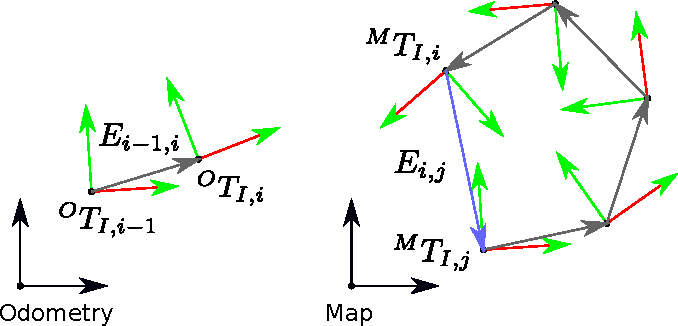
\includegraphics[width=0.5\textwidth]{../figs/graph_slam_residuals.pdf}
  \caption{Residuals used in pose graph optimization.}
  \label{fig:graph_slam_residuals}
\end{figure}
















\section{ポーズグラフの最適化}

\subsection{コスト関数}

ポーズグラフの最適化を考えるために,ポーズグラフ内で定義される残差ベクトルについて考えます.
式(\ref{eq:odometry_edge}),(\ref{eq:loop_edge})に示すように,ポーズグラフにおけるエッジは2つの姿勢間の相対姿勢として定義されます.
このエッジが観測,すなわち固定値であると仮定し,以下の残差ベクトルを定義します.
%
\begin{align}
  {\bf r}_{i, j}({}^{M}T_{I, i}, {}^{M}T_{I, j}) = \left( \log \left( E_{i, j}^{-1} {}^{M}T_{I, i}^{-1} {}^{M}T_{I, j} \right) \right)^{\vee}
  \label{eq:pose_graph_residual}
\end{align}
%
式(\ref{eq:pose_graph_residual})が$i$番目と$j$番目のエッジに対して定まる残差ベクトルとなるため,この総和を最小化する姿勢の集合を求めることでポーズグラフの最適化を行います.
%
\begin{align}
 E \left( \mathcal{T} \right) = \sum_{ i, j \in \mathcal{E} } \rho \left( \left\| {\bf r}_{i, j} \right\|_{ \Omega_{i, j} }^{2} \right)
  \label{eq:pose_graph_cost_function}
\end{align}
%
なお$\left\| {\bf r}_{i, j} \right\|_{ \Omega_{i, j} }^{2} = {\bf r}_{i, j}^{\top} \Omega_{i, j} {\bf r}_{i, j}$は情報行列$\Omega_{i, j}$を用いたマハラノビス距離の2乗を表します.





\subsection{ヤコビアンの計算}

式(\ref{eq:pose_graph_cost_function})のコスト関数を最小化するにあたり,式(\ref{eq:pose_graph_residual})に示す残差ベクトルの${}^{M}T_{I, i}$と${}^{M}T_{I, j}$に関するヤコビアンを求めます.
ヤコビアンの計算のために,$\Delta_{i, j} = E_{i, j}^{-1} {}^{M}T_{I, i}^{-1} {}^{M}T_{I, j}$を導入します.
$\Delta_{i, j}$を用いると,ヤコビアンはそれぞれ連鎖則を用いて以下のように計算できます.
%
\begin{align}
  \begin{split}
    & \frac{ \partial {\bf r}_{i, j} }{ \partial {}^{M}T_{I, i} }
    = \frac{ \partial {\bf r}_{i, j} }{ \partial \Delta_{i, j} }
      \frac{ \partial \Delta_{i, j} }{ \partial {}^{M}T_{I, i} } \\
%
    & \frac{ \partial {\bf r}_{i, j} }{ \partial {}^{M}T_{I, j} }
    = \frac{ \partial {\bf r}_{i, j} }{ \partial \Delta_{i, j} }
      \frac{ \partial \Delta_{i, j} }{ \partial {}^{M}T_{I, j} }
  \end{split}
\end{align}
%
以下,それぞれの微分について考えます.

まず$\partial {\bf r}_{i, j} / \partial \Delta_{i, j}$を考えます.
式(\ref{eq:pose_graph_residual})より,以下の等式が成り立つ$J$を求めれば良いことになります.
%
\begin{align}
  \left( \log \left( \exp \left( \delta \boldsymbol \xi^{\wedge} \right) \Delta_{i, j} \right) \right)^{\vee} - \left( \log \left( \Delta_{i, j} \right) \right)^{\vee} = J \delta \boldsymbol \xi
  \label{eq:deij_dDeltaij_J_deltaxi}
\end{align}
%
ここで$\log \left( \exp \left( \delta \boldsymbol \xi^{\wedge} \right) \Delta_{i, j} \right)$は,BCH展開を用いて以下のように1次近似することができます.
%
\begin{align}
  \left( \log \left( \exp \left( \delta \boldsymbol \xi^{\wedge} \right) \Delta_{i, j} \right) \right)^{\vee}
  \simeq {\bf r}_{i, j} + J_{l}^{-1} \left( {\bf r}_{i, j} \right) \delta \boldsymbol \xi
  \label{eq:bch_1_order_approx}
\end{align}
%
なお,${\bf r}_{i, j} = \left( \log \left( \Delta_{i, j} \right) \right)^{\vee}$であり,$J_{l}( \cdot )$は${\rm SE}(3)$に関する左ヤコビアンと呼ばれ,以下のように定義されます.
%
\begin{align}
  \begin{gathered}
    J_{l}( \boldsymbol \xi )
    = \left( \begin{matrix}
        J_{l}( \boldsymbol \phi ) & 0_{3 \times 3} \\
        Q( \boldsymbol \xi )      & J_{l}( \boldsymbol \phi ) \\
      \end{matrix} \right) \\
%
    J_{l}( \boldsymbol \phi ) = I_{3}
                              + \frac{ 1 - \cos \theta }{ \| \theta \|^{2} } \boldsymbol \phi^{\wedge}
                              + \frac{ \theta - \sin \theta }{ \| \theta \|^{3} } \left( \boldsymbol \phi^{\wedge} \right)^{2} \\
%
    Q( \boldsymbol \xi ) = \frac{1}{2} {\bf v}^{\wedge}
                         + \frac{1 - \alpha}{ \|\boldsymbol \phi \|^{2} } \left( \boldsymbol \phi^{\wedge} {\bf v}^{\wedge} + {\bf v}^{\wedge} \boldsymbol \phi^{\wedge} \right)
                         + \frac{\beta - 1}{ \|\boldsymbol \phi \|^{4} } \boldsymbol \phi^{\wedge} {\bf v}^{\wedge} \boldsymbol \phi^{\wedge} \\
%
    \alpha = \frac{ \sin \theta }{ \theta } \cdot \frac{ \theta + \sin \theta }{ 2 \left( 1 - \cos \theta \right) } \\
%
    \beta = \frac{1}{ \theta^{2} } \left( 1 - \frac{ \sin \theta }{ \theta } \right)
  \end{gathered}
  \label{eq:left_jacobian_se3}
\end{align}
%
ただし,$\boldsymbol \xi^{\wedge} = \left( \left( {\bf v}^{\top} ~ \boldsymbol \phi^{\top} \right)^{\top} \right)^{\wedge} \in \mathfrak{se}(3) $,$\boldsymbol \phi^{\wedge} \in \mathfrak{so}(3)$,$\theta = \| \boldsymbol \phi \|$です\footnote{式(\ref{eq:left_jacobian_se3})には${\rm SE}(3)$と${\rm SO(3)}$の左ヤコビアンがどちらも記載されていますが,引数が$\mathfrak{se}(3)$か$\mathfrak{so}(3)$でそれぞれを区別します.}.
式(\ref{eq:deij_dDeltaij_J_deltaxi}),(\ref{eq:bch_1_order_approx})から,$\partial {\bf r}_{i, j} / \partial \Delta_{i, j}$は以下になります.
%
\begin{align}
  \frac{ \partial {\bf r}_{i, j} }{ \partial \Delta_{i, j} } = J_{l}^{-1}( {\bf r}_{i, j} )
  \label{eq:deij_dDeltaij}
\end{align}
%

次に$\partial \Delta_{i, j} / \partial {}^{M}T_{I, i}$の微分を考えるために,まず$\Delta_{i, j} \left( \delta \boldsymbol \xi \right) = E_{i, j}^{-1} \left( \exp \left( \delta \boldsymbol \xi^{\wedge} \right) {}^{M}T_{I, i} \right)^{-1} {}^{M}T_{I, j}$,$\delta \boldsymbol \xi^{\wedge} \in \mathfrak{se}(3)$を導入します.
この$\Delta_{i, j} \left( \delta \boldsymbol \xi \right)$に左から$\Delta_{i, j}^{-1}$を掛けることで,恒等元$I_{4}$の周辺での変化量を考えます.
%
\begin{align}
  \begin{split}
    \Delta_{i, j}^{-1} \Delta_{i, j} \left( \delta \boldsymbol \xi \right)
%
    = & {}^{M}T_{I, j}^{-1} {}^{M}T_{I, i} E_{i, j} E_{i, j}^{-1} {}^{M}T_{I, i}^{-1} \exp \left( -\delta \boldsymbol \xi^{\wedge} \right) {}^{M}T_{I, j} \\
%
    = & {}^{M}T_{I, j}^{-1} \exp \left( -\delta \boldsymbol \xi \right) {}^{M}T_{I, j} \\
%
    = & \exp \left( \left( -\operatorname{Ad}_{ {}^{M}T_{I, j}^{-1} } \delta \boldsymbol \xi \right)^{\wedge} \right) \\
    \simeq & I_{4} + \left( -\operatorname{Ad}_{ {}^{M}T_{I, j}^{-1} } \delta \boldsymbol \xi \right)^{\wedge}
%
  \end{split}
\end{align}
%
式(\ref{eq:dT_dT})と比較すると,$\partial \Delta_{ij} / \partial {}^{M}T_{I, i}$は以下になることがわかります.
%
\begin{align}
  \frac{ \partial \Delta_{i, j} }{ \partial {}^{M}T_{I, i} } = - \operatorname{Ad}_{ {}^{M}T_{I, j}^{-1} }
  \label{eq:dDeltaij_dTi}
\end{align}
%

以上から,式(\ref{eq:deij_dDeltaij}),(\ref{eq:dDeltaij_dTi})より,$\partial {\bf r}_{i, j} / \partial {}^{M}T_{I, i}$は以下となります.
%
\begin{align}
  \frac{ \partial {\bf r}_{i, j} }{ \partial {}^{M}T_{I, i} } = -J_{l}^{-1}( {\bf r}_{i, j} ) \operatorname{Ad}_{ {}^{M}T_{I, j}^{-1} }
  \label{eq:deij_dTi}
\end{align}
%
なお同様の計算を行うと,$\partial {\bf r}_{i, j} / \partial {}^{M}T_{I, j}$を以下のように導くことができます.
%
\begin{align}
  \frac{ \partial {\bf r}_{i, j} }{ \partial {}^{M}T_{I, j} } = J_{l}^{-1}( {\bf r}_{i, j} ) \operatorname{Ad}_{ {}^{M}T_{I, i} }
  \label{eq:deij_dTj}
\end{align}



\subsection{ガウス・ニュートン法による最適化}

式(\ref{eq:pose_graph_cost_function})に示すコスト関数を最小化するためにも,ガウス・ニュートン法を用います.
まず式(\ref{eq:pose_graph_residual})に示す残差ベクトル${\bf r}_{i, j}$に対する${}^{M}T_{I, i}$,および${}^{M}T_{I, j}$に関するヤコビアンは,それぞれ式(\ref{eq:deij_dTi}),(\ref{eq:deij_dTj})のように定まります.
以下,それぞれのヤコビアンを$J_{i}$,$J_{j}$とします.
今,$i, j$番目のエッジに対して定まる残差ベクトル${\bf r}_{i, j}$に対するヤコビアンを$J_{i, j} = \left( 0 ~ \cdots ~ 0 ~ J_{i} ~ 0 ~ \cdots 0 ~ J_{j} ~ 0 ~ \cdots ~ 0 \right) \in \mathbb{R}^{6 \times 6N}$とします($i, j$番目の残差に影響を与えるのは$i$,$j$番目の姿勢のみのため,それ以外の要素はすべて0になります.).
これを用いて,ヘッセ行列$H \in \mathbb{R}^{6N \times 6N}$,と勾配ベクトル${\bf b} \in \mathbb{R}^{6N}$を求めます.
%
\begin{align}
  \begin{gathered}
    H = \sum_{ ij \in \mathcal{E} } w_{i, j} J_{i, j}^{\top} J_{i, j} \\
    {\bf b} = \sum_{ ij \in \mathcal{E} } w_{i, j} J_{i, j}^{\top} {\bf r}_{i, j} \\
  \end{gathered}
  \label{eq:graph_slam_hessian_gradient}
\end{align}
%
なお,$w_{i, j} = \rho^{\prime} \left( \| {\bf r}_{i, j} \|_{ \Omega_{i, j}^{2} } \right)$です.
このヘッセ行列と勾配を用いて,$H \delta \boldsymbol \xi = -{\bf b}$を満たす$\delta \boldsymbol \xi$を求めます.
$\delta \boldsymbol \xi \in \mathbb{R}^{6N}$は$N$個のブロックで構成されるベクトルとなっており,各ブロックはそれぞれの姿勢に対応する更新量となっています.
つまり$i$番目のブロックのベクトルを$\delta \boldsymbol \xi_{i} \in \mathbb{R}^{6}$とすると,対応する$i$番目の姿勢${}^{M}T_{I, i}$は以下のように更新されます.
%
\begin{align}
  {}^{M}T_{I, i} \leftarrow \exp \left( \delta \boldsymbol \xi_{i}^{\wedge} \right) {}^{M}T_{I, i}
\end{align}
%

グラフベースSLAMを実装するにあたり,ヘッセ行列のサイズは$6N \times 6N$となり,単純に逆行列を求めると計算コストが非常に大きくなってしまいます.
しかし多くの場合,一般的なグラフベースSLAMでは,$H$の対角成分以外のほとんどの成分が0となります.
このような行列は{\bf 疎行列}(Sparse Matrix)と呼ばれ,専用のソルバーを用いると高速に$H \delta \boldsymbol \xi = -{\bf b}$を満たす$\delta {\bf x}$を求めることができます.
そのため,実際には式(\ref{eq:graph_slam_hessian_gradient})に示すような大きなサイズのヤコビアンの計算は行わず,$J_{i}$,$J_{j}$を計算して,行列の各要素に加算していくような計算を行います.













\section{ループ検知}
\label{subsec:gicp}

\subsection{GICPの最適化}

前述の通り,ループ検知のためにはGICPを用います.
GICPはSource点群$\mathcal{P}$とTarget点群$\mathcal{Q}$の2つの点群を照合するために利用できる手法です.
GICPでは,それぞれの点群を正規分布を用いて表現しますが,そのためにまず,各点群の全ての点に対して最近某探索を行い,各点群内から周辺の点を取得します.
そしてそられの点を用いて,平均と共分散行列を計算します.
平均と分散の計算は式(\ref{eq:points_mean}),(\ref{eq:points_covariance})に基づきます.
すなわち,$\mathcal{P}$の$i$番目の点は$\bar{ {\bf p} }_{i}$と$C_{i}^{p}$,$\mathcal{Q}$の$i$番目の点は$\bar{ {\bf q} }_{i}$と$C_{i}^{q}$によりそれぞれ表されます.
GICPでは,これらを用いてコスト関数を以下のように定めます.
%
\begin{align}
  E \left( T \right) = \sum_{i=1}^{N} \rho \left( \left( \bar{ {\bf q} }_{i} - T \bar{ {\bf p} }_{i} \right)^{\top} \left( \hat{C}_{i}^{q} + T \hat{C}_{i}^{p} T^{-1} \right)^{-1} \left( \bar{ {\bf q} }_{i} - T \bar{ {\bf p} }_{i} \right) \right)
  \label{eq:gicp_cost_function}
\end{align}
%
ただし$\hat{C}^{p}$,$\hat{C}^{q}$は以下となります.
%
\begin{align}
  \begin{gathered}
    \hat{C}^{p} = \left( \begin{matrix}
      C^{p}          & {\bf 0} \\
      {\bf 0}^{\top} & 0
    \end{matrix} \right) \in \mathbb{R}^{4 \times 4} \\
%
    \hat{C}^{q} = \left( \begin{matrix}
      C^{q}          & {\bf 0} \\
      {\bf 0}^{\top} & 0
    \end{matrix} \right) \in \mathbb{R}^{4 \times 4}
  \end{gathered}
\end{align}
%

\begin{figure}[!t]
  \centering
  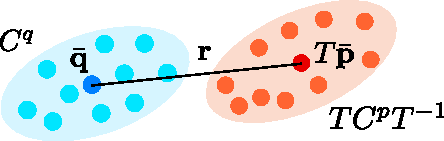
\includegraphics[width=0.3\textwidth]{../figs/gicp_residual.pdf}
  \caption{Residual error used in GICP.}
  \label{fig:gicp_residual}
\end{figure}


本書では,GICPもガウス・ニュートン法を用いて解きますが,表記の簡略化のために,${\bf r}_{i} = \bar{ {\bf q} }_{i} - T \bar{ {\bf p} }_{i}$,$\Omega_{i} = \left( \hat{C}_{i}^{q} + T \hat{C}_{i}^{p} T^{\top} \right)^{-1}$とおきます.
まず${\bf r}_{i}$の$T$に対するヤコビアンを求めるために,以下を満たす$J_{i}$を求めます.
%
\begin{align}
  \bar{ {\bf q} }_{i} - \exp \left( \delta \boldsymbol \xi^{\wedge} \right) T \bar{ {\bf p} }_{i} - \left( \bar{ {\bf q} }_{i} - T \bar{ {\bf p} }_{i} \right) = J_{i} \delta \boldsymbol \xi
  \label{eq:gicp_jacobi_approx}
\end{align}
%
式(\ref{eq:gicp_jacobi_approx})の左辺を展開すると,以下が得られます.
%
\begin{align}
  \begin{split}
    -\exp \left( \delta \boldsymbol \xi^{\wedge} \right) T \bar{ {\bf p} }_{i} + T \bar{ {\bf p} }_{i}
%
    = & - \left( \exp \left( \delta \boldsymbol \xi^{\wedge} \right) - I_{4} \right) T \bar{ {\bf p} }_{i} \\
%
    = & - \left( \begin{matrix}
            \delta \boldsymbol \phi^{\wedge} & \delta {\bf v} \\
            {\bf 0}^{\top}                   & 0
          \end{matrix} \right)
          \left( \begin{matrix}
            \bar{ {\bf p} }_{i}^{'} \\
            1
          \end{matrix} \right) \\
%
    = & - \left( \begin{matrix}
            - \left( \bar{ {\bf p} }_{i}^{'} \right)^{\wedge} \delta \boldsymbol \phi + \delta {\bf v} \\
            0
          \end{matrix} \right) \\
%
    = & \left( \begin{matrix}
          -I_{3}         & \left( \bar{ {\bf p} }_{i}^{'} \right)^{\wedge} \\
          {\bf 0}^{\top} & {\bf 0}^{\top}
        \end{matrix} \right) \delta \boldsymbol \xi \\
  \end{split}
\end{align}
%
ただし,$\bar{ {\bf p} }_{i}^{'} = R \bar{ {\bf p} }_{i} + {\bf t}$としています.
よって,式(\ref{eq:gicp_jacobi_approx})を満たす$J_{i}$は以下になります.
%
\begin{align}
  J_{i} = \left( \begin{matrix}
            -I_{3}         & \left( \bar{ {\bf p} }_{i}^{'} \right)^{\wedge} \\
            {\bf 0}^{\top} & {\bf 0}^{\top}
          \end{matrix} \right)
  \label{eq:gicp_jacobian}
\end{align}
%
このヤコビアンを用いて,ヘッセ行列と勾配を以下のように求めます.
%
\begin{align}
  \begin{gathered}
    H = \sum_{i=1} w_{i} J_{i}^{\top} \Omega_{i} J_{i} \\
    {\bf b} = \sum_{i=1} w_{i} J_{i}^{\top} \Omega_{i} {\bf r}_{i} \\
  \end{gathered}
  \label{eq:gicp_hessian_and_gradient}
\end{align}
%
なお$w_{i} = \rho^{\prime} \left( {\bf r}_{i} \Omega_{i} {\bf r}_{i} \right)$です.
この$H$と${\bf b}$を用いて,$H \delta \boldsymbol \xi = -{\bf b}$を満たす$\delta \boldsymbol \xi$を求め,$T \leftarrow \exp \left( \delta \boldsymbol \xi^{\wedge} \right) T$で姿勢を更新します.

式(\ref{eq:gicp_hessian_and_gradient})の導出について簡単に述べますが,これは\ref{subsec:gauss-newton_method}節でも述べたように,状態が微小変化した際の残差ベクトルの線形近似を用いたコスト関数について考えることで導出できます.
%
\begin{align}
  \sum_{i=1}^{N} \left( {\bf r}_{i} + J_{i} \delta \boldsymbol \xi \right)^{\top} \Omega_{i} \left( {\bf r}_{i} + J_{i} \delta \boldsymbol \xi \right)
  =
  \sum_{i=1}^{N} {\bf r}_{i}^{\top} \Omega_{i} {\bf r}_{i} + 2 \delta \boldsymbol \xi^{\top} \Omega_{i} J_{i} {\bf r}_{i} + \delta \boldsymbol \xi^{\top} J_{i}^{\top} \Omega_{i} J_{i} \delta \boldsymbol \xi
\end{align}
%
この右辺を$\delta \boldsymbol \xi$で微分して{\bf 0}とすると以下が得られます(ただし式(\ref{eq:gicp_hessian_and_gradient})と比較して,下の式では$w_{i}$が抜けていることに注意してください).
%
\begin{align}
  \sum_{i=1}^{N} J_{i}^{\top} \Omega_{i} J_{i} \delta \boldsymbol \xi = -\sum_{i=1}^{N}  J_{i}^{\top} \Omega_{i} {\bf r}_{i}
\end{align}
%



\subsection{ループ検知の成功判定}

ループ検知のためにGICPを用いて,式(\ref{eq:gicp_cost_function})に示すコスト関数の最小化を行い,点群の照合を行います.
この照合結果を基にループ検知の成功・失敗を判断する必要があるのですが,点群の照合の是非を明示的に示す指標を作成することは困難です.
例えば,最終的なコスト関数の値,もしくは残差の平均値が一定以下になっているというような閾値は,ある程度の精度で照合の是非を判定できますが,必ずしも判断の正しい指標になるとはいえません.
しかし実装においては,これらの指標を用いるのが有用な場合が多くあります.
本書で紹介している実装では,残差の平均値や,照合率(最近傍点との距離が閾値以下の点の割合)などに閾値を定め,これらに基づきループ検知が成功したかどうかの判定を行っています.

ただしこのような方法では,照合に失敗した場合でも成功したと判定してしまう場合があります.
このような誤った情報がグラフに組み込まれると,グラフの最適化が破綻してしまうこともあります.
そのため式(\ref{eq:graph_slam_hessian_gradient})に示すように,グラフの最適化においてもフーバー損失等のロバストカーネルを利用することが有効になります.











\section{座標変換の計算と地図構築}

\subsection{座標変換}

LIOを用いると,オドメトリ座標上でのIMUの姿勢${}^{O}T_{I}$が得られます.
またポーズグラフの最適化を実行すると,新しく検出されたキーフレームの位置が修正され,それが地図座標上でのIMUの姿勢${}^{M}T_{I}$となります.
この2つの姿勢を用いて,図\ref{fig:frames}に示す地図とオドメトリ座標間の変換${}^{M}T_{O}$を求めるにあたり,図\ref{fig:map_odom_transformation}ように,地図座標上のIMUの姿勢,およびオドメトリ座標上でのIMUの姿勢が一致するとします.
するとこの関係から,${}^{M}T_{O}$を以下のように求められます.
%
\begin{align}
  \begin{split}
    {}^{M}T_{O} = & {}^{M}T_{I} {}^{O}T_{I}^{-1} \\
                = & {}^{M}T_{I} {}^{I}T_{O}
  \end{split}
\end{align}
%
なお本書で詳細は述べませんが,自己位置推定をする場合でも同じように${}^{M}T_{O}$を求めます.

\begin{figure}[!t]
  \centering
  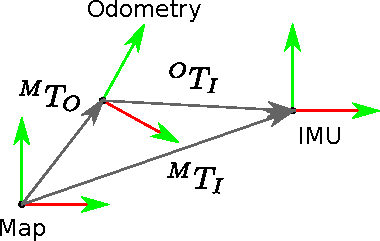
\includegraphics[width=0.3\textwidth]{../figs/map_odom_transformation.pdf}
  \caption{Residuals used in pose graph optimization.}
  \label{fig:map_odom_transformation}
\end{figure}



\subsection{地図構築}

ポーズグラフの最適化が終わると,地図座標上での各キーフレームが${}^{M}T_{I, i}$修正されます.
これらの姿勢,および各キーフレームに対応する点群${}^{I}\mathcal{P}_{i}$を用いて,以下のように点群地図を構築します.
%
\begin{align}
  {}^{M}\mathcal{M} = \bigcup_{i=1}^{K} \bigcup_{{}^{I}{\bf p} \in {}^{I}\mathcal{P}_{i}} {}^{M}T_{I, i} {}^{I}{\bf p}
\end{align}
%
ここで$K$はキーフレームの数です.
ただし本書で紹介しているグラフベースSLAMでは,この地図点群が処理に利用されることはありません.
そのため,SLAMプロセス終了時に一度実行するだけでも問題はありません.
ポーズグラフの最適化後に都度実行すると,地図が正しく構築できているかをオンラインで確認することができるため,本書で紹介する実装では最適化後に毎回実行しています.





\section{実用にあたって}

本章で紹介した方法では,移動量に対して閾値を設けてキーフレームを検出し,そのキーフレームに対応するLiDARの観測点群を保存しておき,この点群をキーフレームに合わせて座標変換することで地図の作成を行いました.
この方法を採用すると,LiDARが計測した全ての点群を用いて地図の作成を行わくなるため,地図点群の密度が低下するという問題が発生してしまいます.
点群の密度を上げるために,例えば一定時間LiDARの計測点群を蓄積したらキーフレームとして検出するという方法も考えられますが,この方法を用いると時間経過とともに使用するメモリ容量が増大してしまいます.
一方で移動量に対して閾値を設けてキーフレームを検出する方法であれば,移動量に対してメモリ容量が増大するため,メモリ効率は優れるというトレードオフがあります.


もし単に点群密度の高い地図を作りたというだけであれば,SLAMを用いて地図を作成した際に使用した同じデータを用いて,その地図上で再度位置推定を実行し,その位置推定結果を基に点群をマッピングするという方法もあります.
少し面倒にはなりますが,この方法であればメモリコストを気にせずに高密度の点群地図が作成することができます.
ただし点群データの全体的な整合性を考えてマッピングされた結果とはならないため,確実に正確な地図が得られる保証がないことには留意しなければなりません.

本章で紹介した方法は,ポーズグラフを用いたグラフベースSLAMになります.
ポーズグラフを用いる場合,LiDARの点群データは最適化対象にならなくなるため,マッピングの精度は通常のグラフベースSLAMと比較すると低下してしまいます.
ただし,通常グラフベースSLAMでは,メモリコストの問題があるため,LiDARが計測した点群すべてを最適化対象にはせず,特徴点やランドマークをLiDARの点群から検出し,これらの位置を最適化対象に加えます.
そのため,特徴点やランドマークの検出性能,またそれらの対応付けの性能がマッピングの精度にも影響することになります.
近年の3D LiDARは観測距離も長く,点群の密度も高いため,単純に2つの計測データを照合するだけでも,高い精度で相対位置を知ることができます.
そのため,このような前提であれば,ポーズグラフの最適化だけでも十分な精度の地図を得られることが多いです.
ただし,文献\cite{}に見られるように,地図全体を最適化するというプロセスを踏むと,より地図の精度を向上させることもできるため,ポーズグラフの最適化だけで十分な精度が得られるかどうかはケースバイケースであるといえます.

本章で述べた方法では,ループ検知を行うために,単純に近隣のキーフレーム間でスキャンマッチングを行うという方法を用いています.
\ref{sec:scan_matching_実用にあたって}でも述べましたが,スキャンマッチングが正しく機能する前提の1つに初期姿勢がある程度正確に取得できてることが挙げられます.
ただしオドメトリでは,移動に対する累積(ドリフト)誤差が無視できないため,SLAM実行中の移動量が長くなるにつれ,ループ検知を行うためのスキャンマッチングの初期姿勢の精度が低下してしまいます.
そのため,単純にスキャンマッチングを用いてループ検知を行うだけでは,大きなループを閉じることができない場合もあります.
そのような場合には,例えばLiDARの計測点群から特徴点や特徴量を抽出し,複数の点群から類似性の高い点群を検出するという方法を用いなければなりません.
ただしこのような方法は,スキャンマッチングでループを検出するより,一般的に精度が低下してしまうことが多いです.
そのため,ポーズグラフの最適化時におけるアウトライアの検出なども考慮する必要が発生することもあります.

なおスキャンマッチングを用いてループ検出を行う場合だけでも,正しくループが閉じることができてれば,オドメトリによる累積誤差が補正できていることを意味します.
そのため,ループが閉じやすいような経路を考えてデータを取得することで,地図作成を成功させるということも実用的にはあります.
ただしループが大きすぎる場合は性能の限界があるため,違う方法の導入を検討しなければなりません.









% \balance
\bibliographystyle{unsrt}
\bibliography{root.bib}


\end{document}
